\documentclass[12pt]{article}
\usepackage[english]{babel}
\usepackage[numbers]{natbib}
\usepackage{graphicx}
\usepackage{sectsty}
\usepackage{float}
\usepackage[table]{xcolor}
\usepackage{tabularx}
\usepackage{arydshln}
\usepackage{fancyhdr}

\fancyhf{}
\bibliographystyle{apalike}
\setcitestyle{open={[},close={]}}
\sectionfont{\color{DarkBlue}} 
\subsectionfont{\color{LightBlue}}
\subsubsectionfont{\color{LightBlue}}
\paragraphfont{\color{LightBlue}}
\subparagraphfont{\color{LightBlue}}
\setlength{\arrayrulewidth}{1pt}
\renewcommand{\arraystretch}{1.5}
\newcolumntype{Y}{>{\centering\arraybackslash}X}
\definecolor{dkgreen}{rgb}{0,0.6,0}
\definecolor{gray}{rgb}{0.5,0.5,0.5}
\definecolor{mauve}{rgb}{0.58,0,0.82}
\definecolor{nicegreen}{rgb}{0.58, 0.98, 0.71}

\definecolor{cgcgrey}{RGB}{229,229,229}
\definecolor{vehiclered}{RGB}{255,187,177}
\definecolor{bigbrotheryellow}{RGB}{255,236,169}
\definecolor{stationorange}{RGB}{255,219,169}
\definecolor{tokenpurple}{RGB}{249,210,222}
\definecolor{kioskgreen}{RGB}{199,232,172}
\definecolor{protocolblue}{RGB}{193,228,247}

\begin{document}
\definecolor{DarkBlue}{HTML}{4a5a8a} 
\definecolor{LightBlue}{HTML}{4f81bf}
\begin{titlepage}
    \begin{flushleft}
        \vspace{1cm} \Huge  \textbf{Cretaceous Gardens Controller}\\
        \vspace{1cm} \Huge  \textit{Software Architecture Design}\\
        \vspace{1cm} \Large \textit{SAD Version 4.0}\\
        \vspace{5cm} \LARGE         Team \#3\\ 
                                    5 December 2019
        \vfill       \Huge  \textbf{CS 460 Software Engineering}
    \end{flushleft}
\end{titlepage}
\normalsize 
\tableofcontents
\pagebreak

\section{Introduction} \label{intro}
\paragraph{} Good software is identified by the end user for its features and functionality, by the client
for its profitability and maintainability, and by the programmer for its legibility and clarity. It should be clear
that all three pillars ultimately characterize good software, but more importantly that the three are interdependent.
The developer must therefore guarantee all of the above for the sake of all entities involved. A top down approach has been
followed thus far. The Technical Feasibility Study posited and answered the fundamental question: Can it be done? The Requirements
Definition Document was then passed the baton and answered the next question: Within what parameters can it be done? Then, 
the Software Requirements Specification document sought to answer: What is the desired behavior of the system? Now this document 
seeks to answer the following: What design will guarantee the desired behavior in a manner that is clear, maintainable, extensible, 
and pragmatic?

\paragraph{} The ultimate goal is to ensure an efficient, safe, and maintainable implementation of the Cretaceous Gardens Controller 
(CGC) software. To that end, all objects are illustrated in their proper contexts, and their crucial 
functions have been delineated as clearly as possible while simultaneously allowing the programmer enough flexibility so 
as to not stifle his or her creative process. 

\paragraph{} This document is a road map for the eventual implementation of the system and details the most 
relevant objects and their relationships in the form of diagrams. Explanations accompany all diagrams for the sake of clarity.
Section \ref{over} presents an overview of the intended design, with descriptions of the largest subsystems that compose the CGC. 
Section \ref{specs} provides greater detail with respect to the individual components and their sub components. Section \ref{samp} 
provides a number of use cases for the system, which have been classified into a few categories. Section \ref{cons} delineates 
constraints to which the design is subject. The implementation plan can be found in Section \ref{impl}. Section \ref{defs} closes the document with the definitions of any terms used throughout the document that may need further clarification.
\footnote{Introduction by Ezequiel Ramos.}.

\section{Design Overview} \label{over}
\paragraph{} The design aims to maximize efficiency and maintainability for the sake of
safety, as it may be compromised by unnecessary component delay or by the degree to which 
lends itself to programmer errors. Objects with red upper left corners execute on their own threads, 
red arrows indicate objects that may trigger events in response to external signals, stacks of objects 
represent multiple instances, and virtual devices are have icons in their lower right corners. 
\footnote{Diagrams by Siri, Anas, and Zeke.}.

\begin{figure}[H]
    \centering
    \textbf{Cretaceous Gardens Controller Overview}\par
    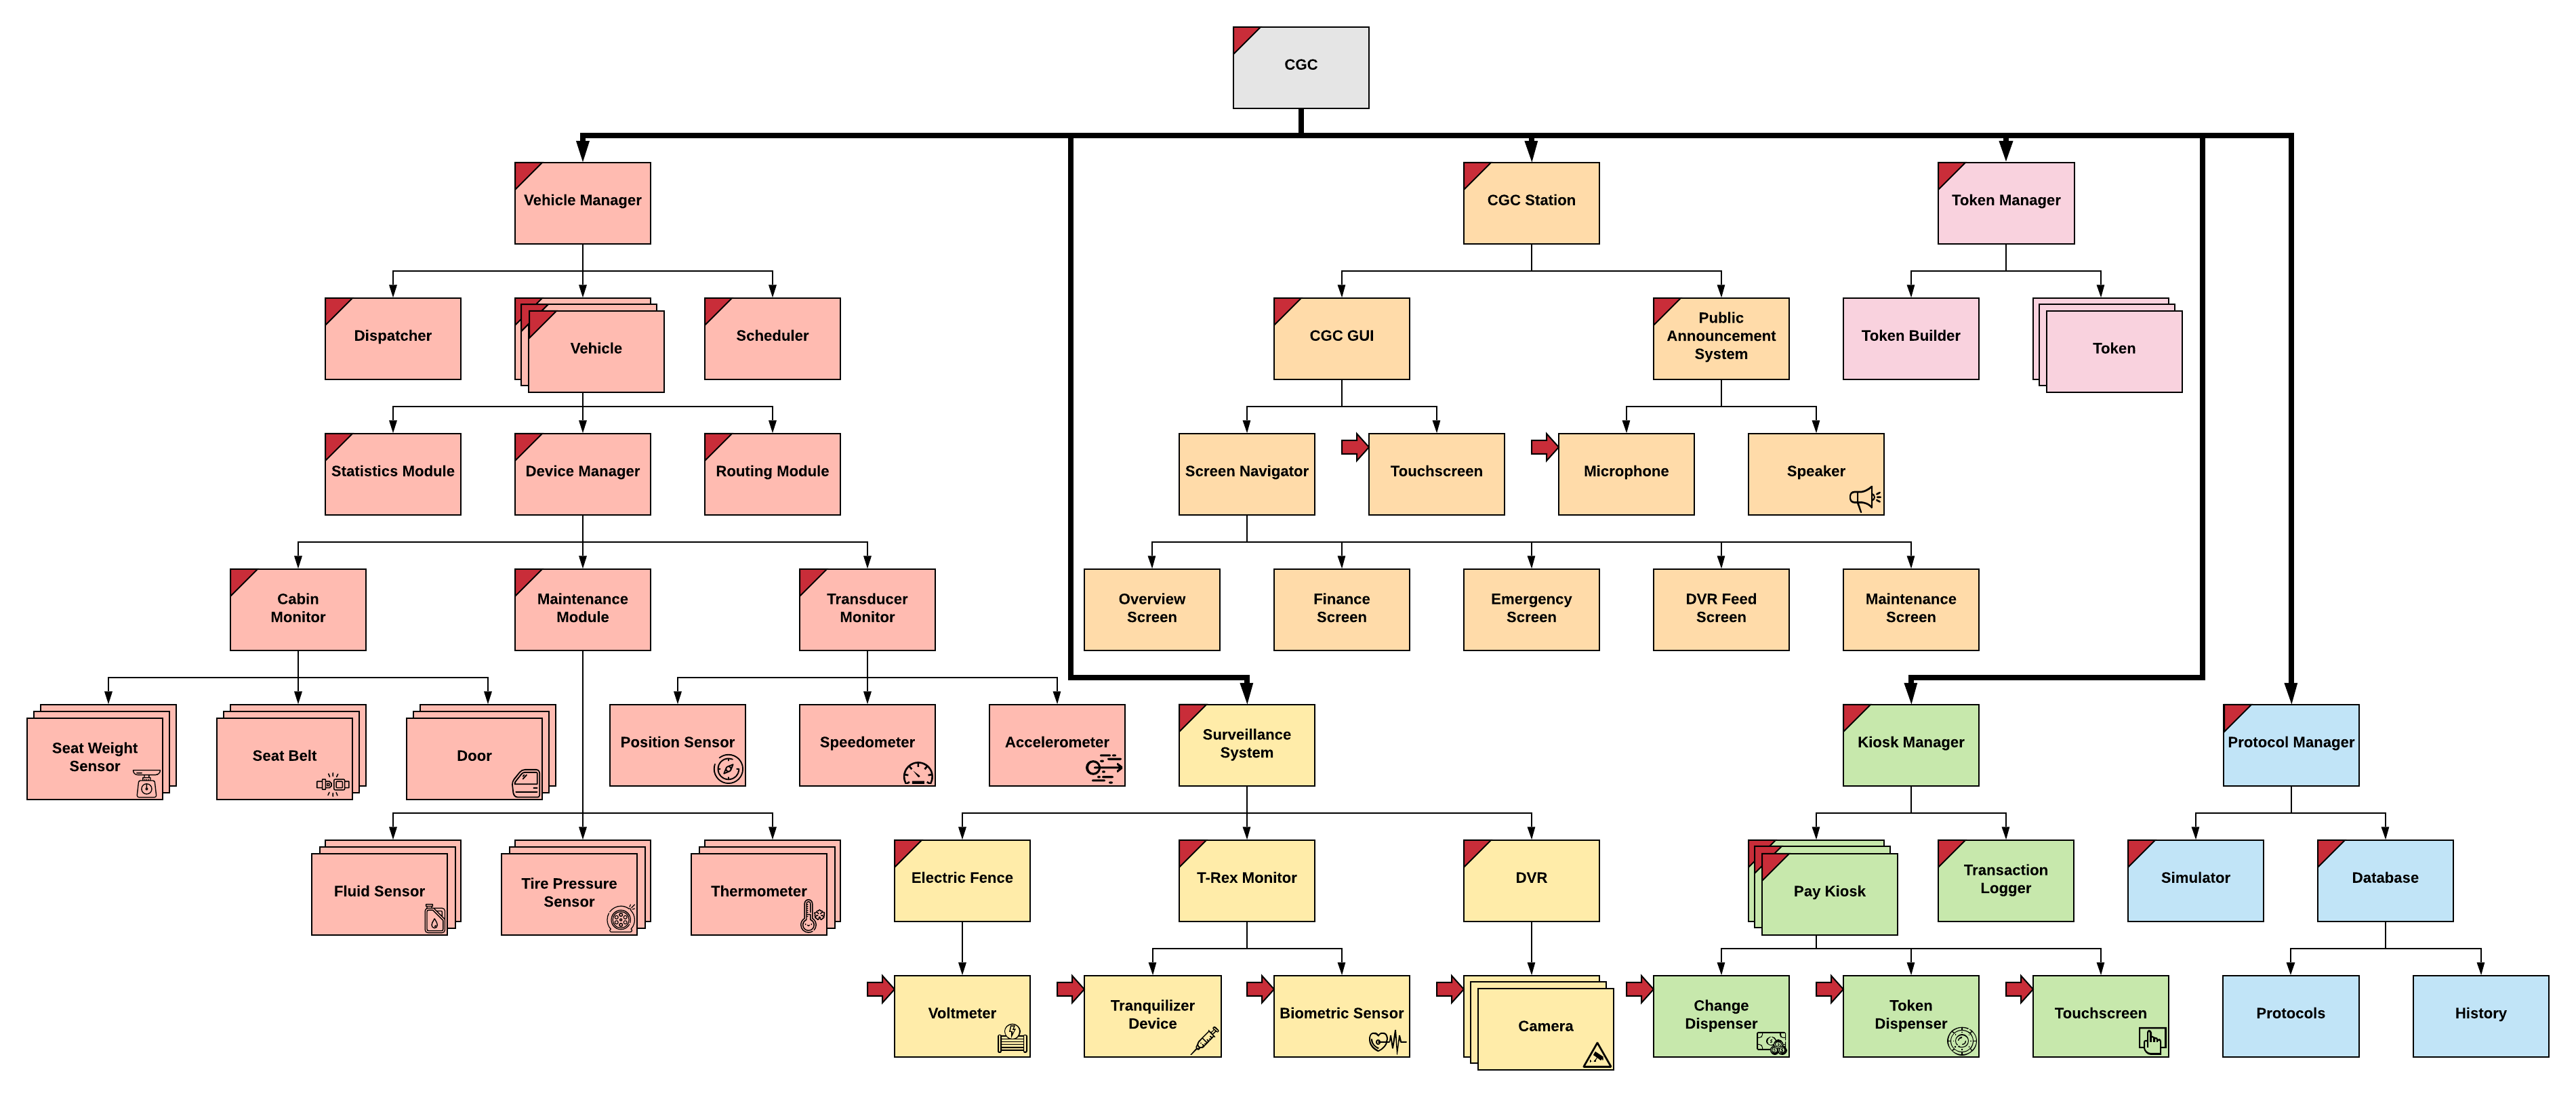
\includegraphics[scale=0.173]{CGC-Design-Overview.png}
    \caption{The CGC is a centralized system that communicates with all active systems. 
    It is not composed of other modules, but rather owns references to all active systems in order to monitor 
    them and to bridge their connections.}
  \label{fig:CGCOverview}
\end{figure}    

\begin{figure}[H]
    \centering
    \textbf{The CGC and its Children}\par
    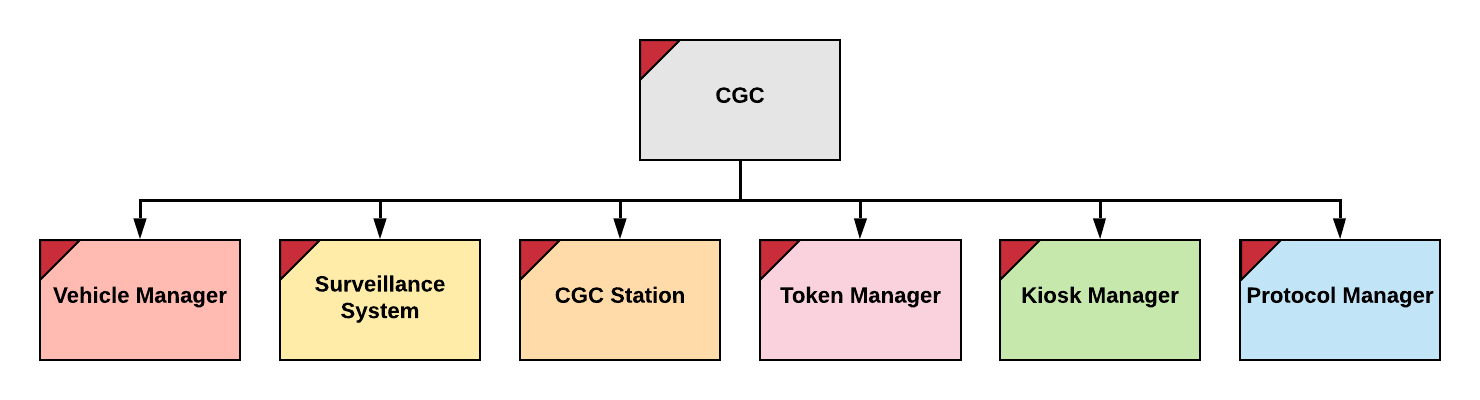
\includegraphics[scale=.23]{CGC-Top.png}
    \caption{The \textbf{CGC} mitigates communication between the \textbf{Vehicle Manager},
    \textbf{Surveillance System}, \textbf{GCG Station}, \textbf{Token Manager}, \textbf{Kiosk Manager}, and \textbf{Protocol Manager}.
    the last of these will not be implemented.}
    \label{fig:CGCTop}
\end{figure}

\begin{figure}[H]
    \centering
    \textbf{Vehicle Manager}\par
    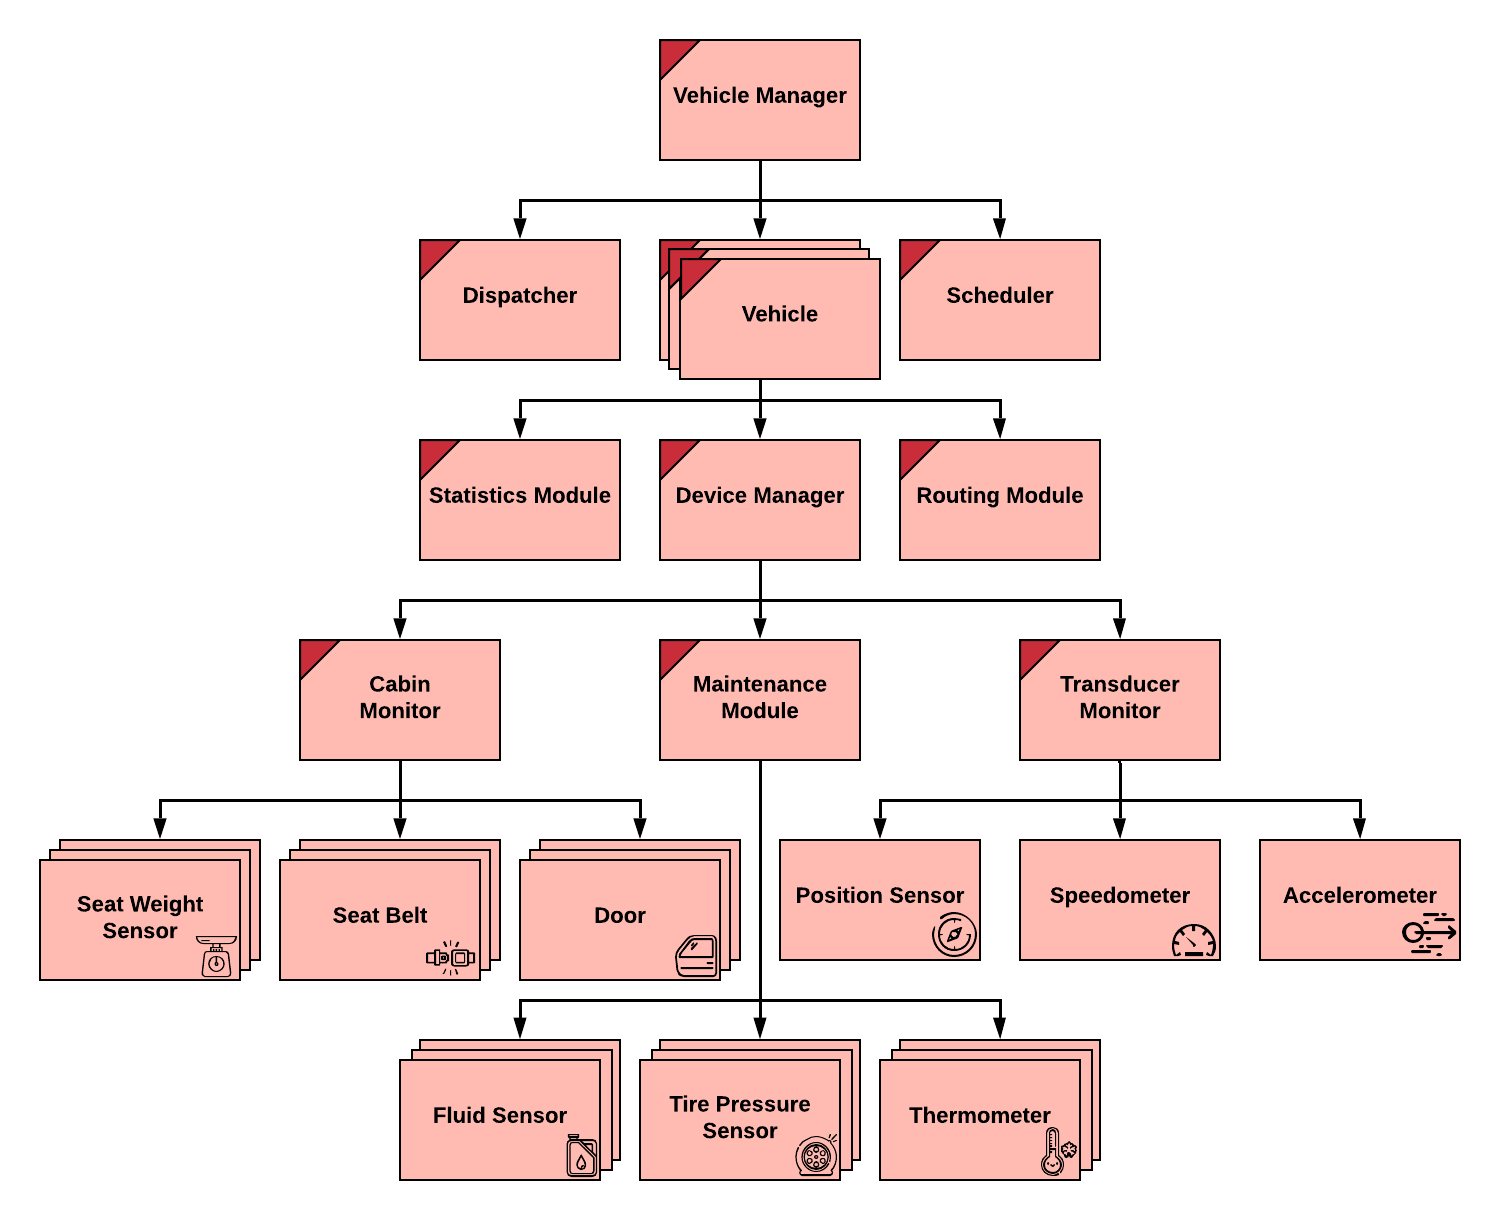
\includegraphics[scale=.23]{Vehicle-Manager.png}
    \caption{The \textbf{Vehicle Manager} coordinates vehicles and vehicle information for the CGC. It communicates 
    directly with the virtual analog of all cars in the system to process hardware, maintenance, and routing information.}
    \label{fig:VehicleManager}
\end{figure}

\begin{figure}[H]
    \centering
    \textbf{Surveillance System}\par
    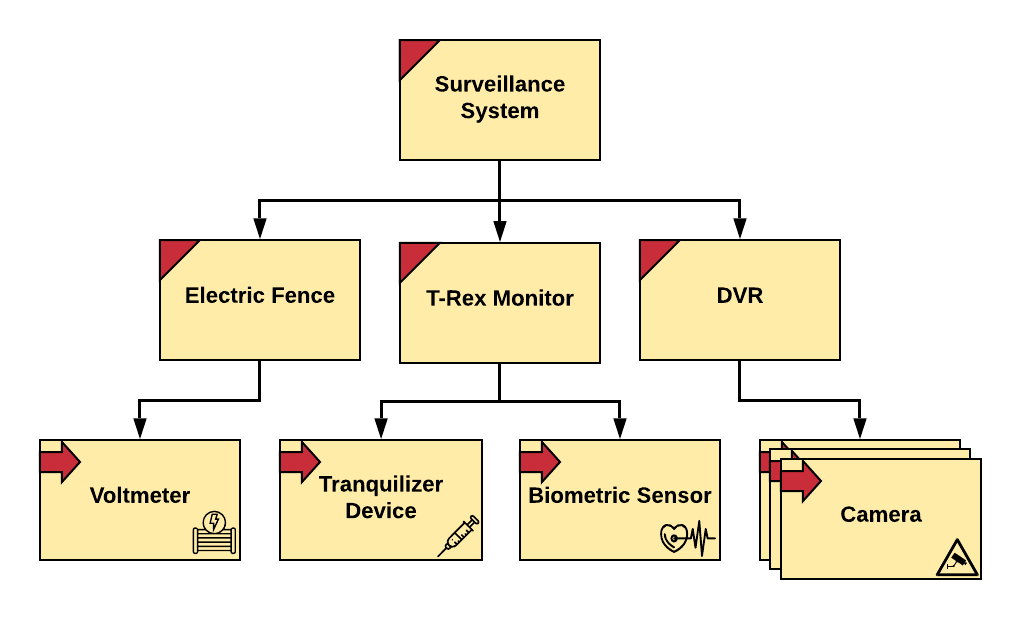
\includegraphics[scale=.27]{Surveillance-System.png}
    \caption{The \textbf{Surveillance System} encapsulates the \textbf{Camera} network (shown as a stack), the \textbf{Electric Fence}, and the
    \textbf{T-Rex Monitor}.}
    \label{fig:SurveillanceSystem}
\end{figure}

\begin{figure}[H]
    \centering
    \textbf{CGC Station}\par
    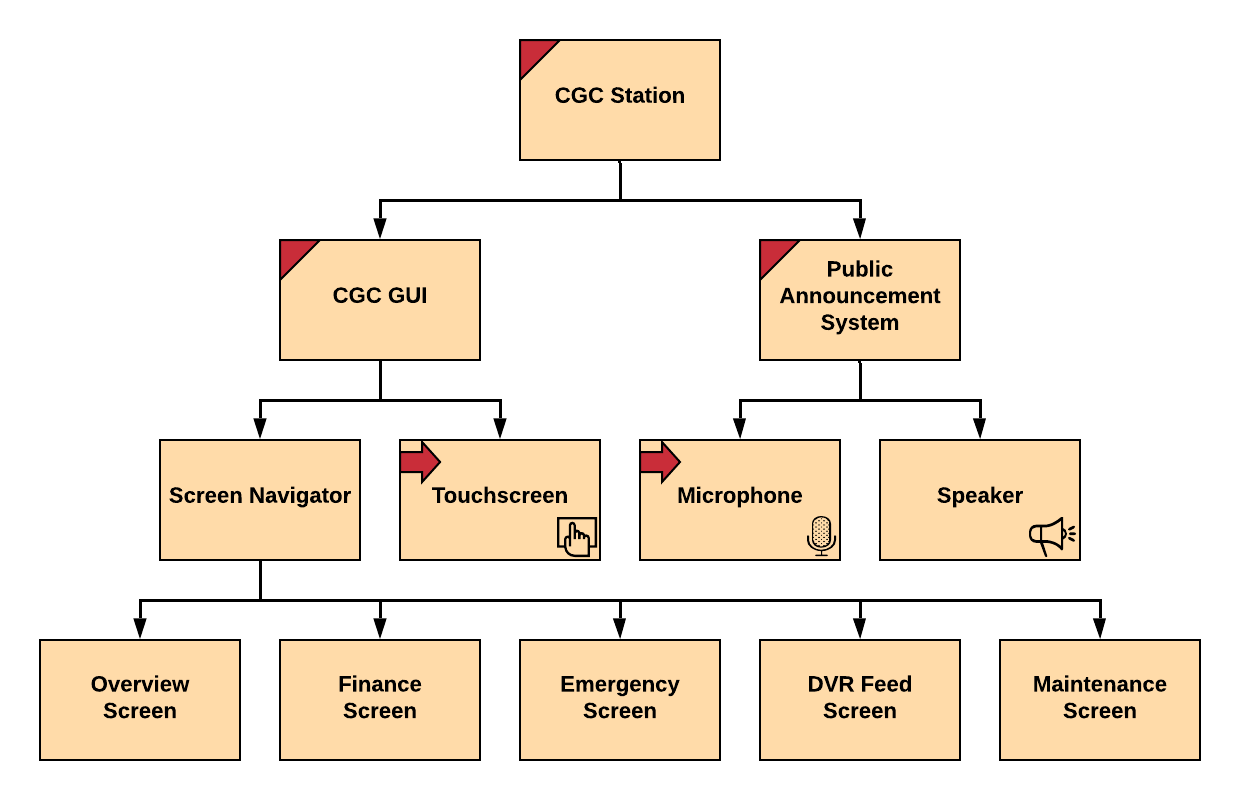
\includegraphics[scale=.28]{CGC-Station.png}
    \caption{The \textbf{CGC Station} represents the means through which the CGC may be accessed by employees. 
    Its three main components are the graphical user interface, the touch screen on which said GUI displays, and
    an intercom system.}
    \label{fig:CGCStation}
\end{figure}

\begin{figure}[H]
    \centering
    \textbf{Token Manager}\par
    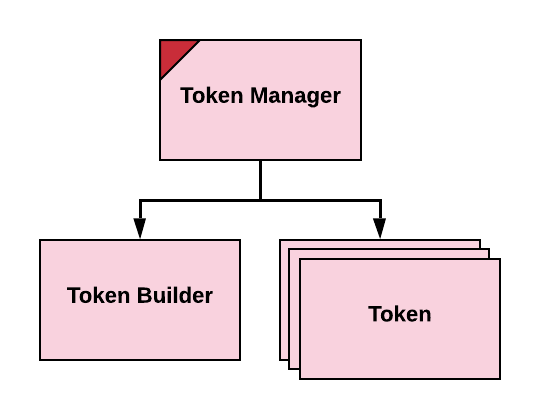
\includegraphics[scale=.40]{Token-Manager.png}
    \caption{The \textbf{Token Manager} is responsible for programming and tracking tokens for the CGC. It communicates 
    directly with the virtual analog of the physical token devices.}
    \label{fig:TokenManager}
\end{figure}

\begin{figure}[H]
    \centering
    \textbf{Protocol Manager}\par
    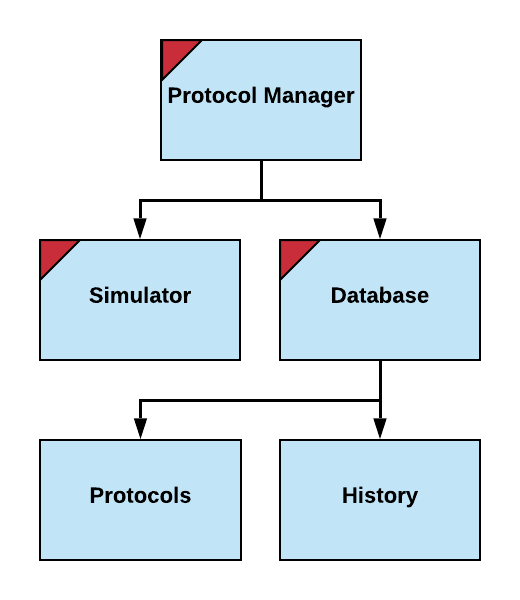
\includegraphics[scale=.30]{Protocol-Manager.png}
    \caption{The \textbf{Protocol Manager} is the component from which the CGC, in effect, receives its overall behavior.
    Because it will not be fully implemented, it will not feature the ability to be given protocols and will instead simply
    contain the \texttt{NormalMode} and \texttt{EmergencyMode} protocols.}
    \label{fig:ProtocolManager}
\end{figure}
  

%\begin{figure}[H]
%    \centerline{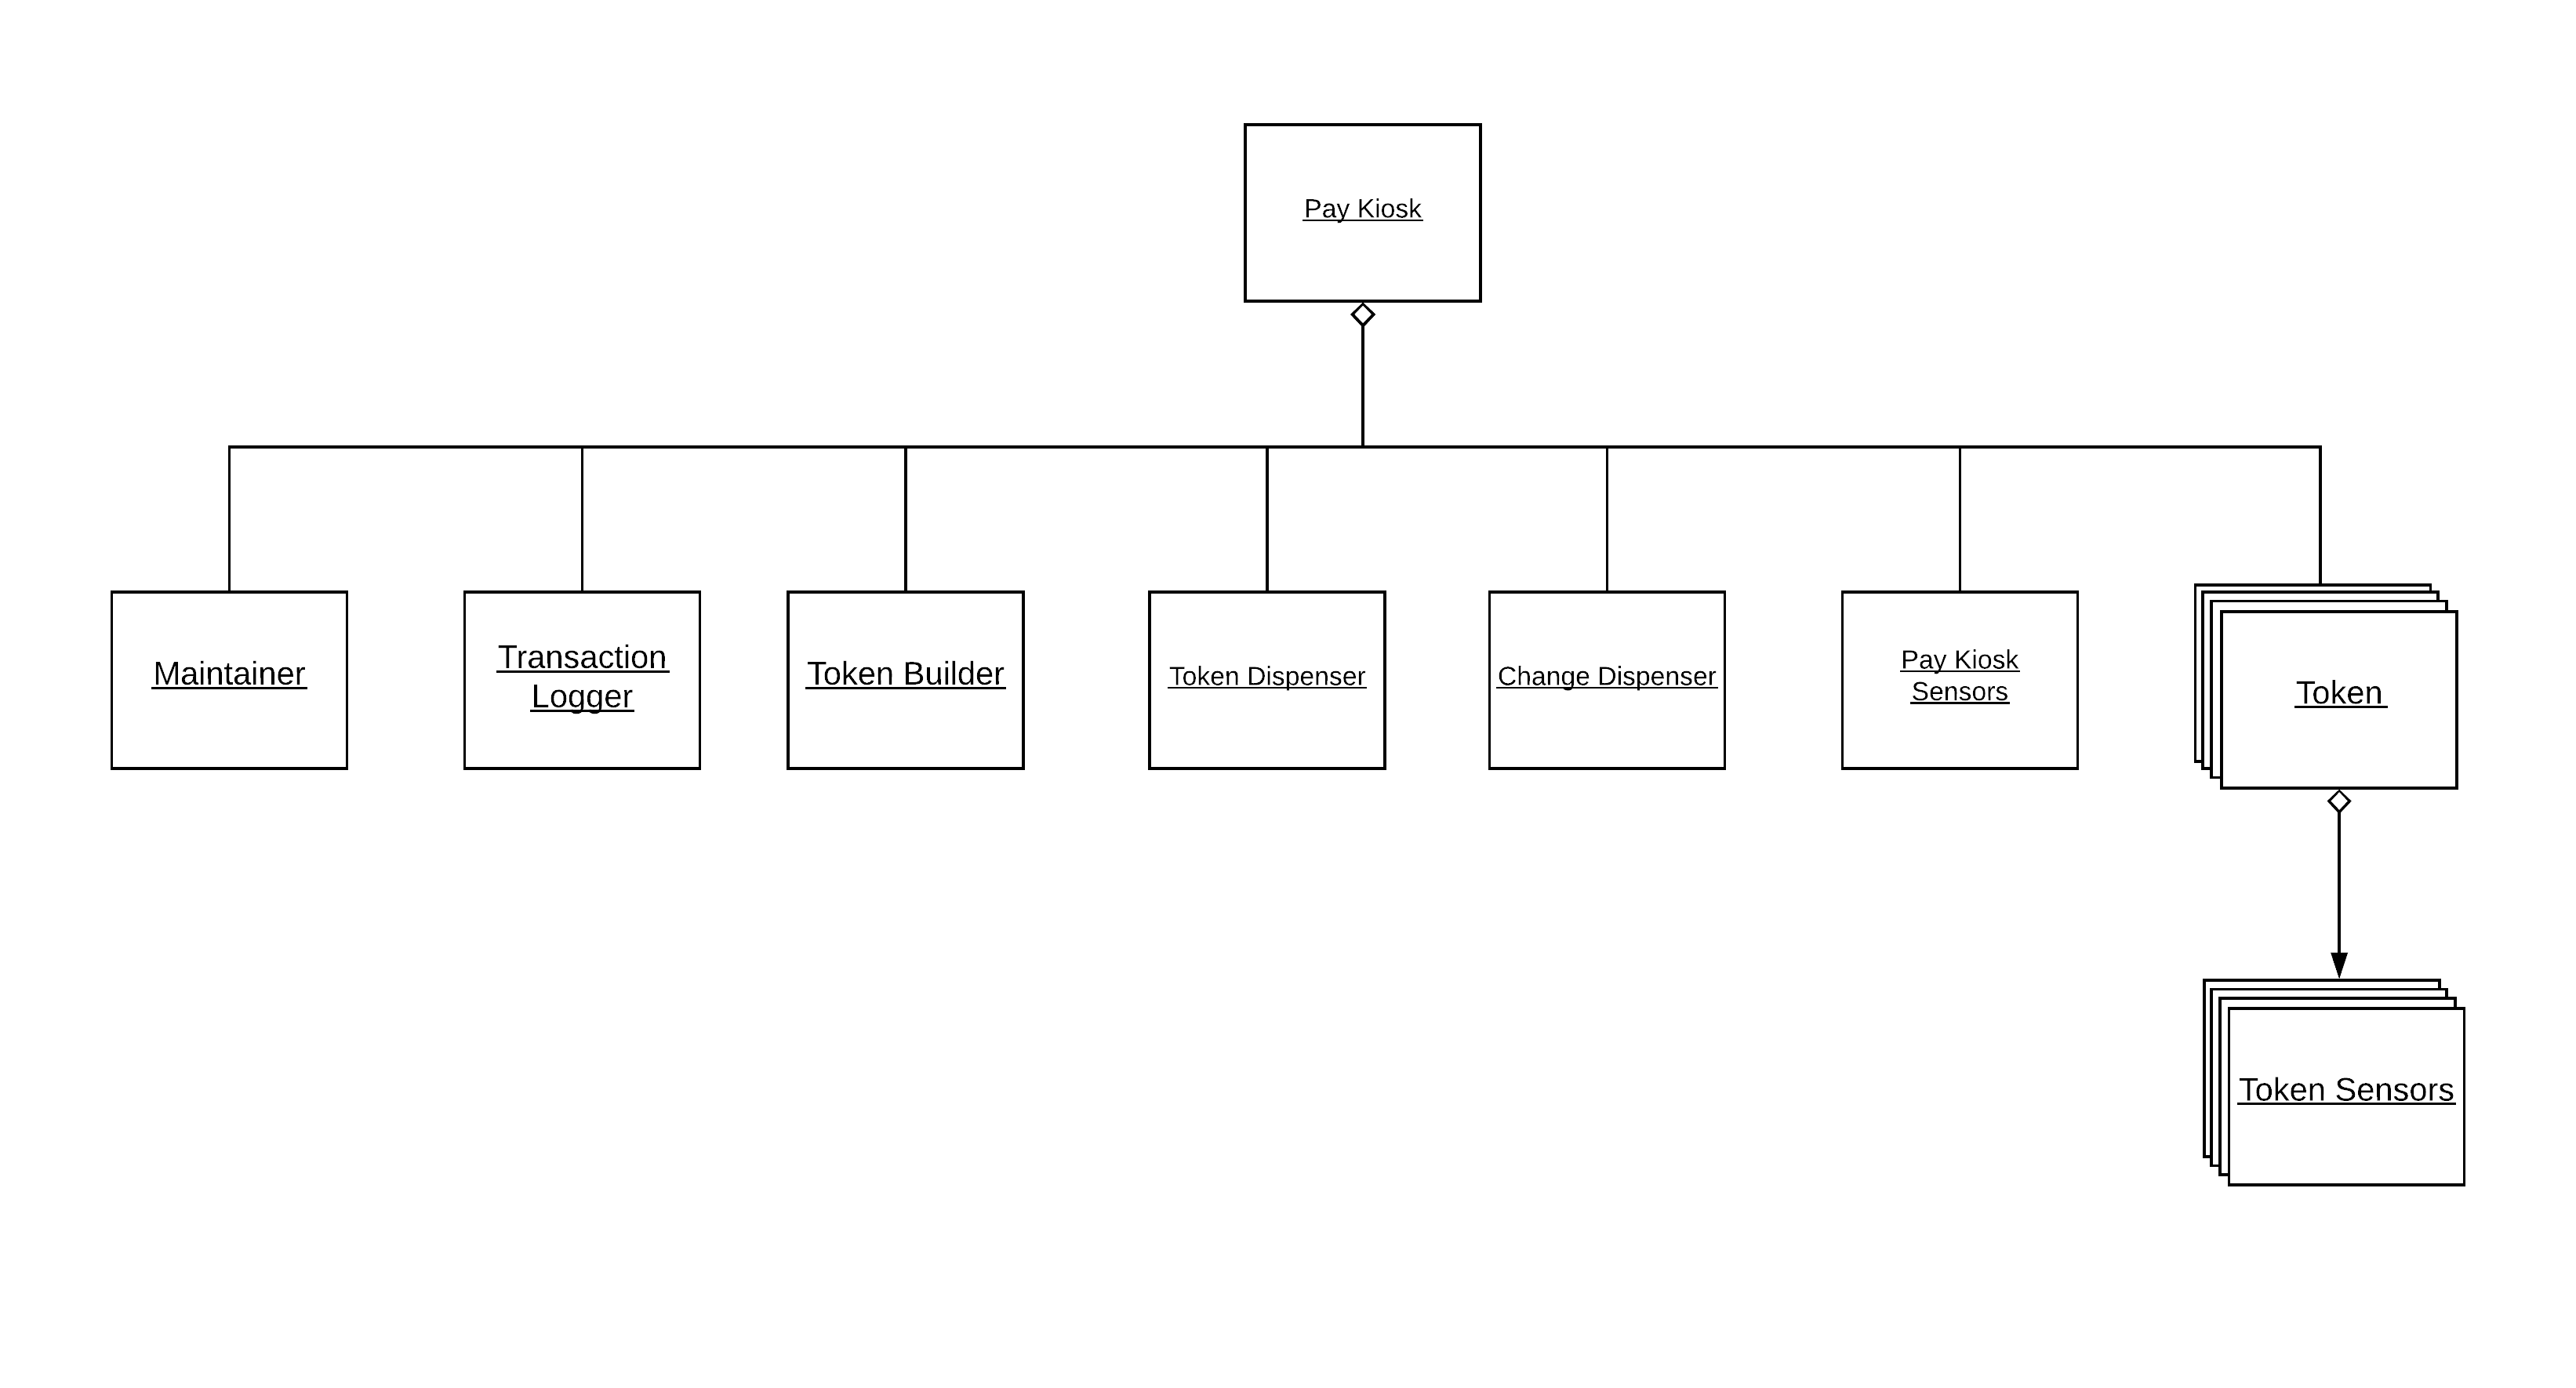
\includegraphics[scale=.20]{PayKiosk.png}}
%    \caption{\textbf{The Pay Kiosk: }The Pay Kiosk object controls the Pay Kiosk device. These are devices used to 
%purchase and build access Tokens for the visitors. It is critical as it helps the users get into 
%the Gardens while also helping the client make money. It is composed of objects that are hardware such
% as the token and change dispensers. it also contains other sensors such as credit card and cash 
% receptacles as well as a touch screen. It has a system that helps log transactions and build tokens. 
% It will configure another critical device, the Token. this is a high tech piece of equipment that is 
% used by the visitor as an access card, but also a communication device, a GPS device, as well as 
% other interactive capabilities.}
%    \label{fig:PayKiosk}
%\end{figure} 

%\begin{figure}[H]
%    \centerline{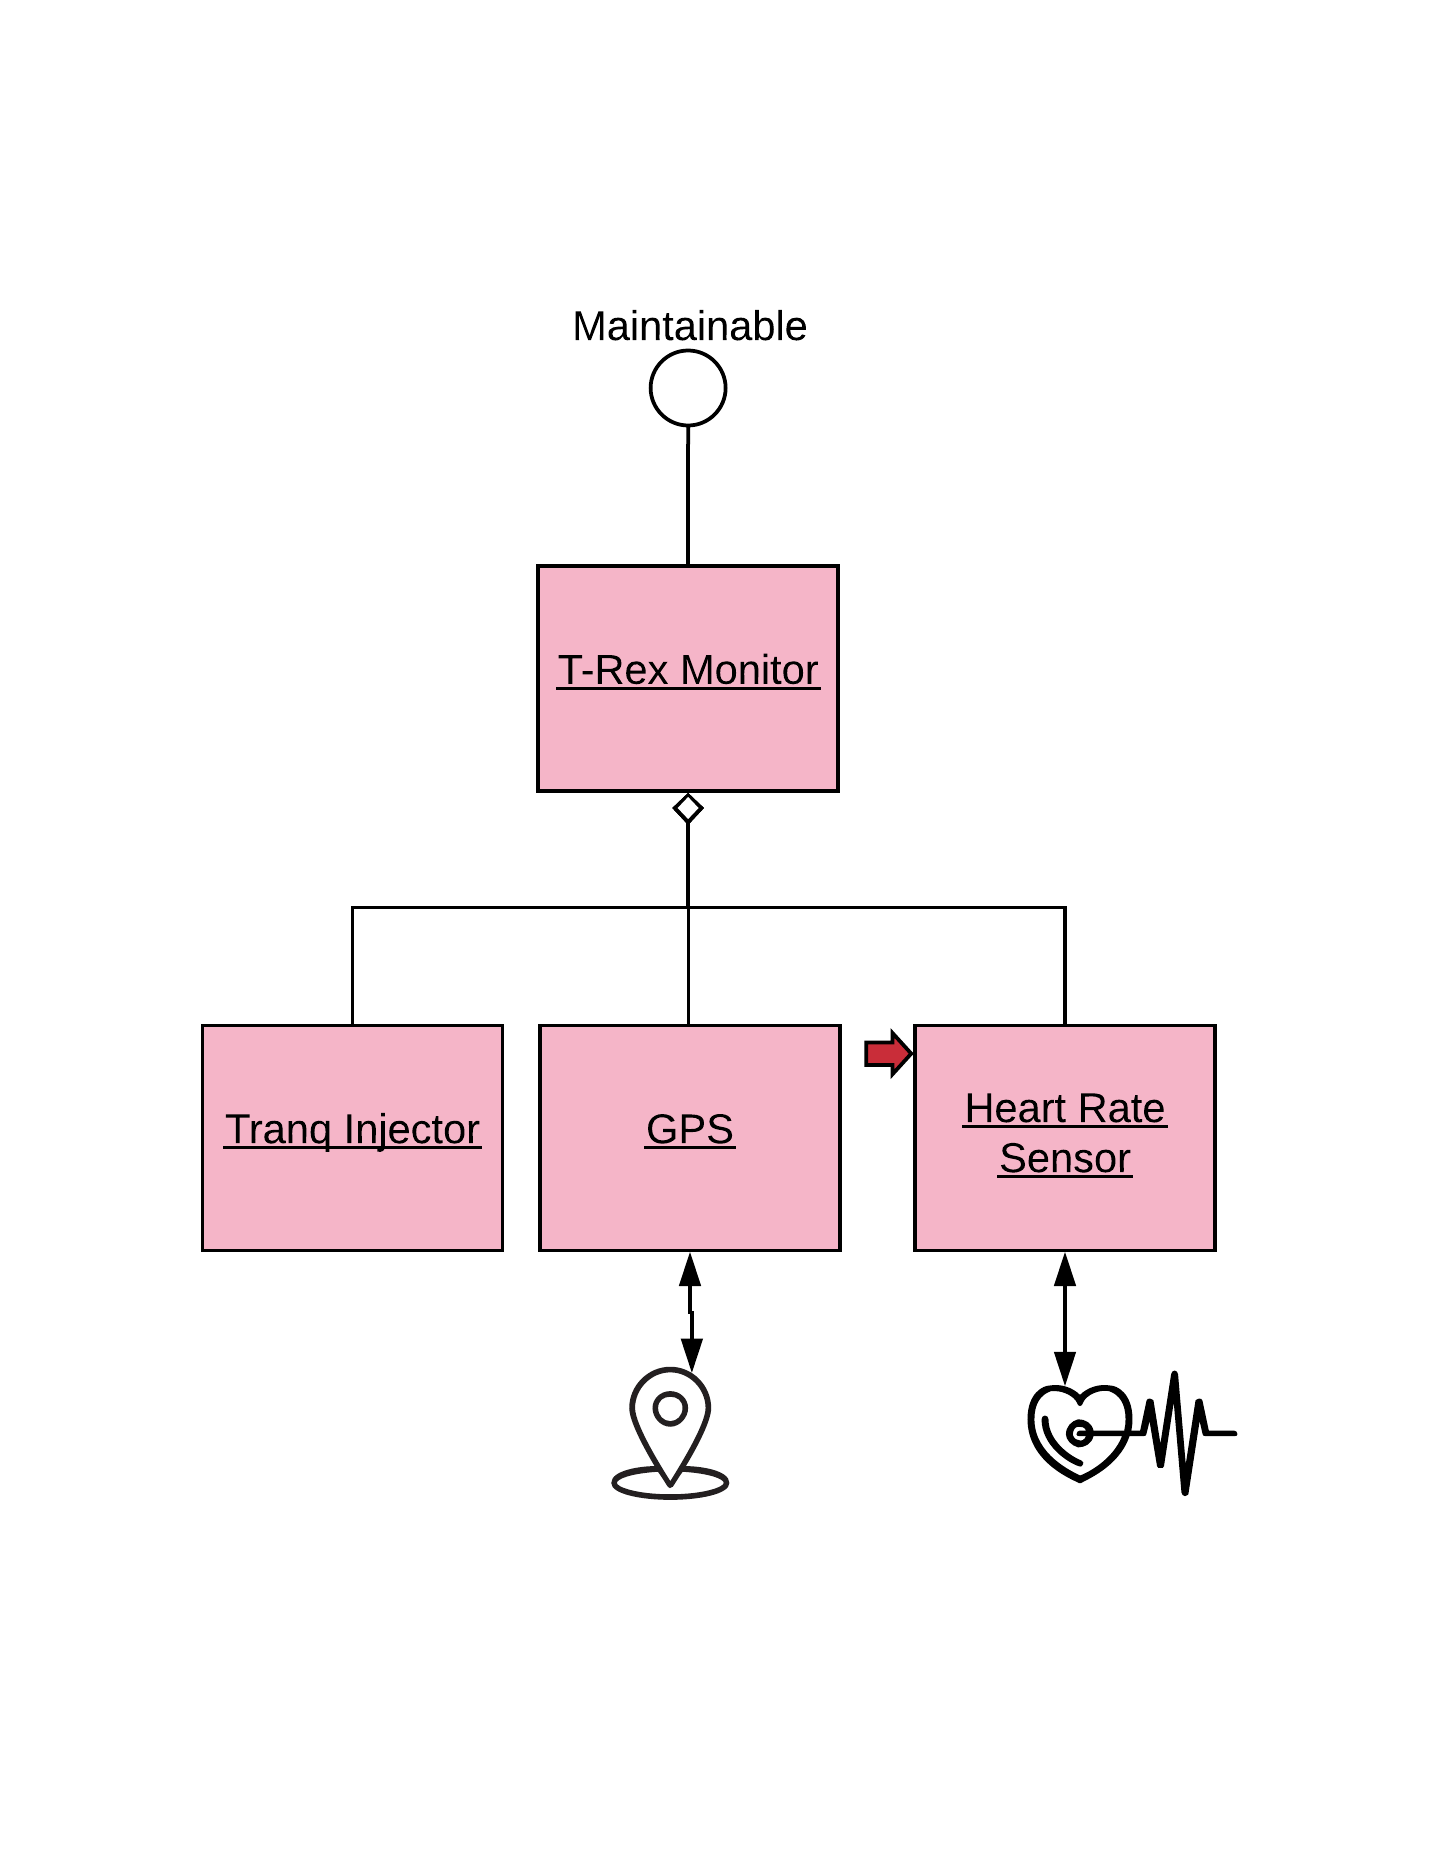
\includegraphics[scale=.20]{TRexMonitor.png}}
%    \caption{\textbf{The T-Rex Monitor: }The T-Rex Monitor  helps the CGC keep track of the T-Rex. 
%It monitors it's Biometrics to make sure it is not stressed out. it also controls a tranquilizer 
%that can put the dino to sleep in a safe manner. This is another Maintainable system. }
%    \label{fig:TRexMonitor}
%\end{figure}    
%
%\begin{figure}[H]
%    \centerline{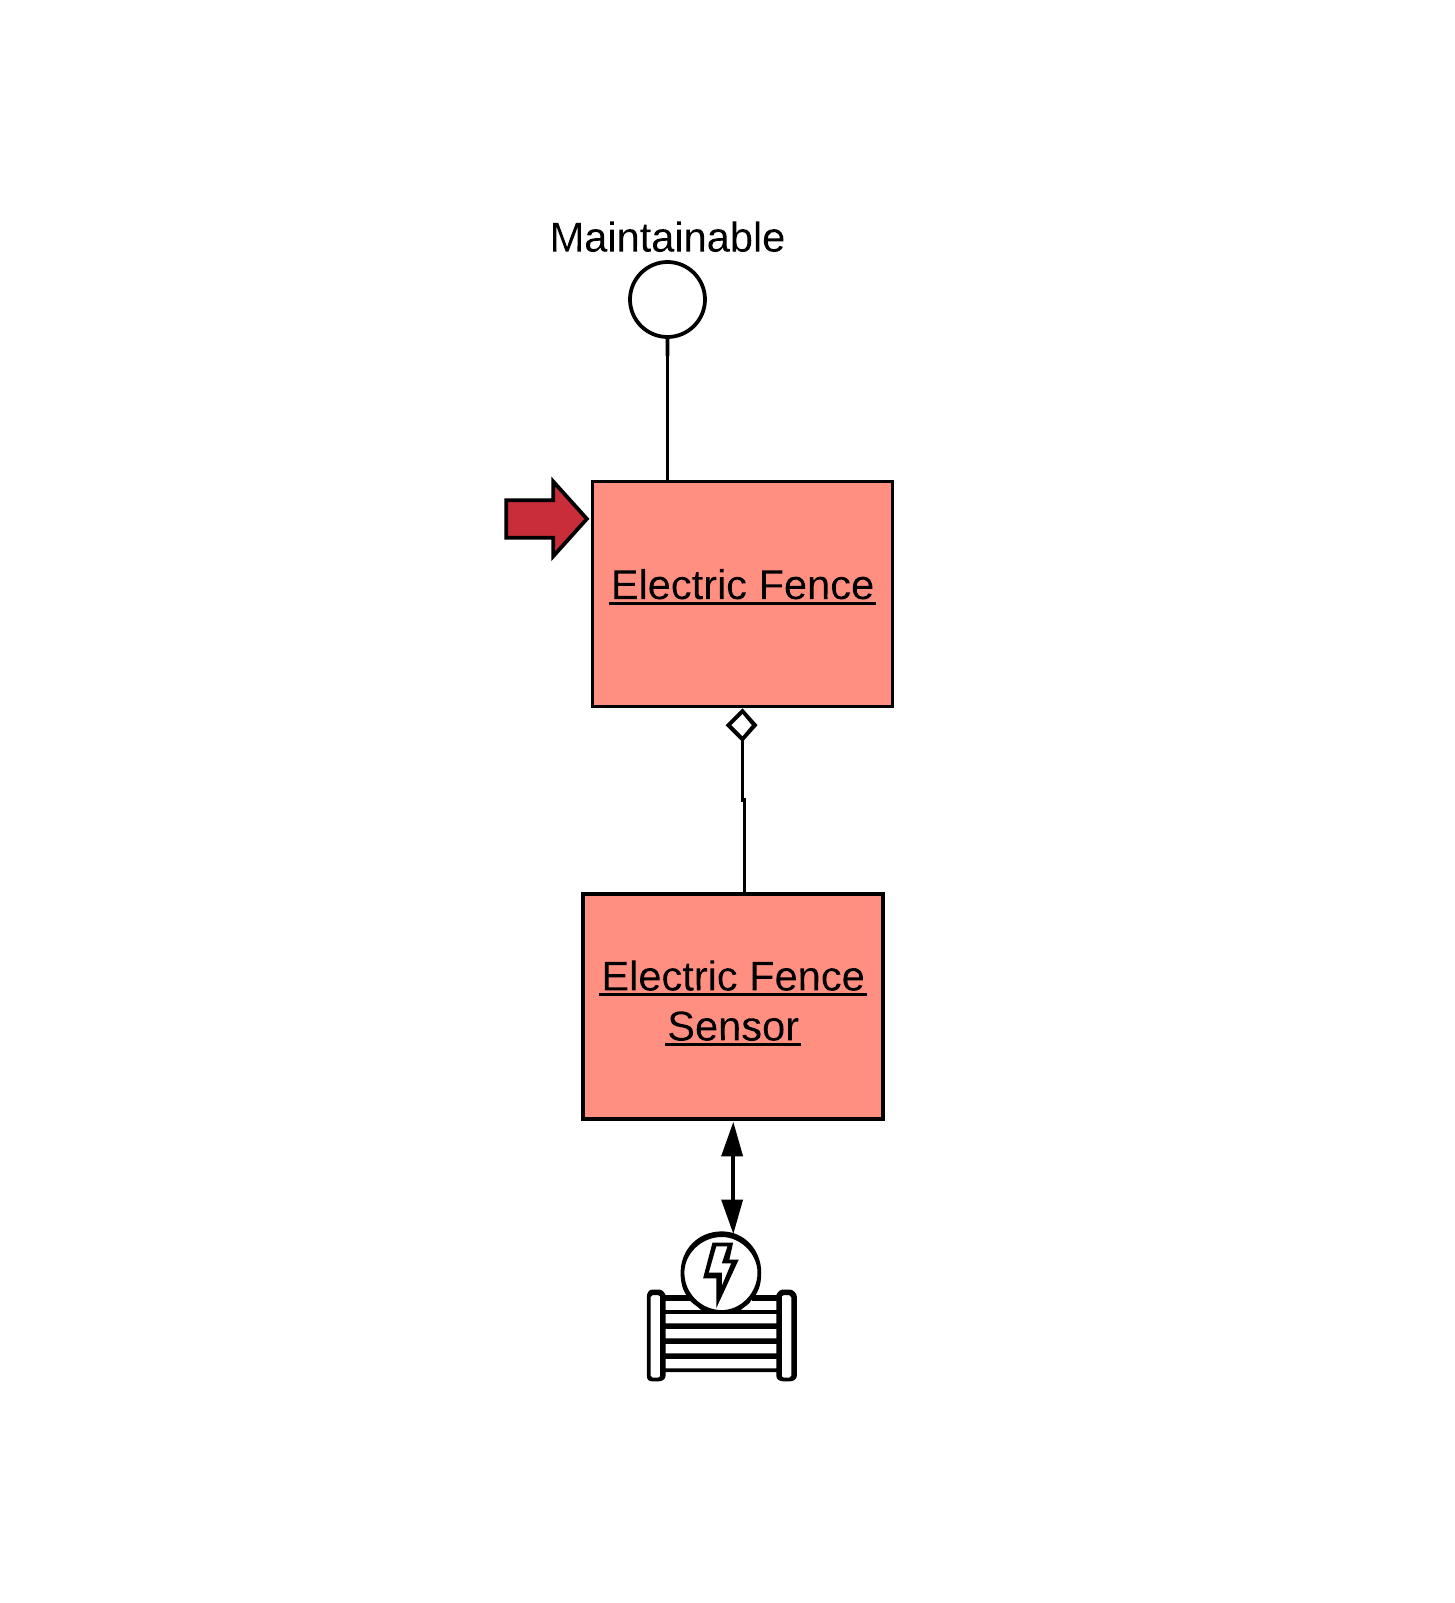
\includegraphics[scale=.20]{ElectricFence.png}}
%    \caption{\textbf{The Electric Fence: }The is another very simple software system. The entire goal is to monitor the 
%electric fence. To do this it utilizes the Electric Fence Sensor. It is also Maintainable.}
%    \label{fig:ElectricFence}
%\end{figure}   
%
%
%\begin{figure}[H]
%    \centerline{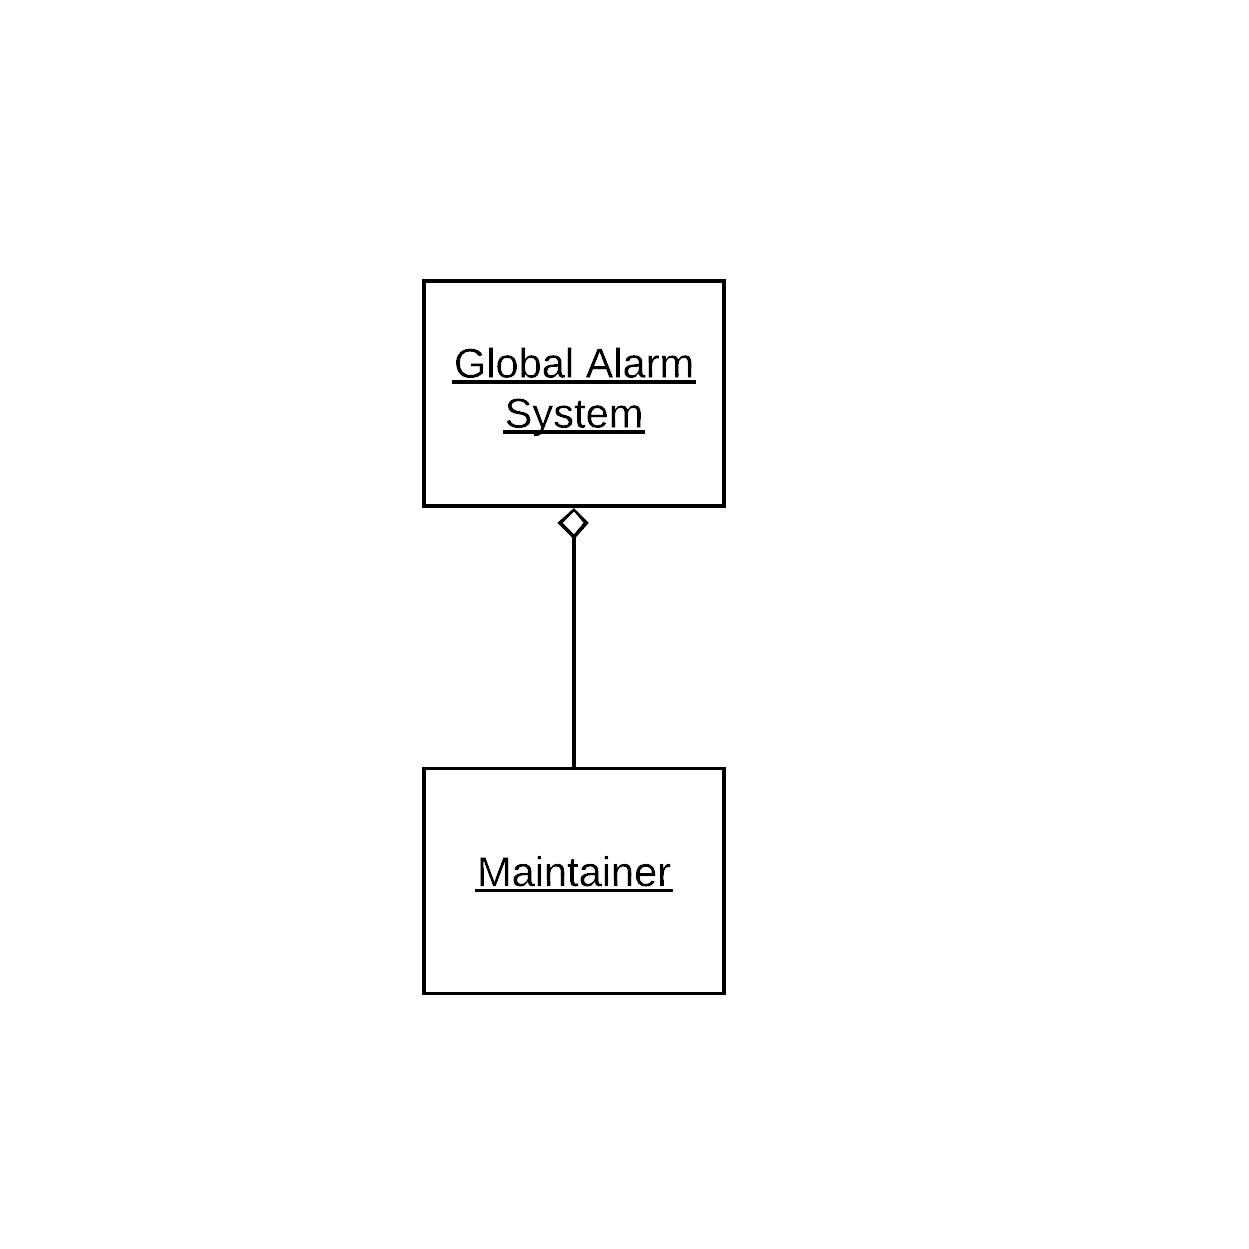
\includegraphics[scale=.20]{GlobalAlarm.png}}
%    \caption{\textbf{The Global Alarm System: }The global alarm system controls the loud PA speakers on the island and is critical
% in case of an emergency. This will be able to report on its health by implementing the maintainable 
% interface. It is very basic and the CGC can broker connections to it from CGC Stations.}
%    \label{fig:GlobalAlarm}
%\end{figure}

\section{Component Specifications} \label{specs}
\paragraph{} \textit{Here are the class specifications\footnote{Component specifications by Anas and Siri.} for objects 
found in Section \ref{over}. The most important attributes and functions are given and where appropriate.}

\subsection*{Cretaceous Gardens Controller}
%%%%%%% intro if necessary
%\begin{table}[H]
%\small
%\begin{tabularx}{\hsize}{|X|X|}
%    \hline
%    \rowcolor{cgcgrey}
%    \multicolumn{2}{|c|}{\textbf{CGC}} \\
%    \hline
%    \hline
%    \multicolumn{2}{|c|}{\textbf{Attributes}}      \\
%    \hline
%    \texttt{messages} & number of registered tokens. \\
%    \texttt{station} & boolean station status \\
%    \texttt{kioskManager} & number of active kiosks  \\
%    \texttt{vehicleManager} &  number of active cars\\
%    \texttt{surveillanceSystem} & things \\
%    \hline
%    \multicolumn{2}{|c|}{\textbf{Functions}} \\
%    \hline
%    \texttt{logTransaction(transaction)} & $\rightarrow$ write to finance controller. \\
%    \texttt{queryFinanceState(SQLScript)} & $\rightarrow$ query financial data. \\
%    \texttt{queryHealthState(SQLScript)} & $\rightarrow$ query health data \\
%    \texttt{getAllGPSLocations()} & $\rightarrow$ get all current GPS locations. \\
%    \texttt{registerToken(tokenID) } & $\rightarrow$ register token. \\
%    \texttt{retireToken(tokenID)} & $\rightarrow$  remove token from registered list\\
%    \texttt{relayStream(cameraID,stationID)} & $\rightarrow$ relay video stream to station\\
%    \texttt{enterEmergencyMode()} & $\rightarrow$ enter emergency mode\\
%    \texttt{enterNormalMode()} & $\rightarrow$ enter normal mode\\
%    \texttt{activateCar()} & $\rightarrow$ activate new car from parking lot\\
%    \texttt{bridgeIntercom(carID,stationID)} & $\rightarrow$ open communication link\\
%    \texttt{connectToPA(stationID)} & $\rightarrow$ connects station to island speakers\\
%    \hline
%
%\end{tabularx}
%\end{table}
%
%
%\subsection{Vehicle Manager}
%%%%intro if necessary
%\begin{table}[H]
%\begin{tabularx}{\hsize}{|X|X|}
%    \hline
%    \rowcolor{vehiclered}
%    \multicolumn{2}{|c|}{\textbf{\texttt{Vehicle}}} \\
%    \hline
%    \hline
%    \multicolumn{2}{|c|}{\textbf{Attributes}}      \\
%    \hline
%    \textbf{isActivated} & Specifies if the car is activated \\
%    \textbf{isParked} & Specifies if the car is parked \\
%    \textbf{Position} & Specifies where is the car located \\
%    \textbf{Destiny} & Destiny where the car has to travel\\
%    \textbf{Passengers} & Number of passengers in the car\\
%    \hline
%    \multicolumn{2}{|c|}{\textbf{Functions}} \\
%    \hline
%    \textbf{checkPosition()} & $\rightarrow$ Return the position of the car in the island \\
%    \textbf{checkIfParked()} & $\rightarrow$ Return if the car is parked \\
%    \textbf{isActivated()} & $\rightarrow$ Return if the car is activated \\
%    \textbf{activateCar()} & $\rightarrow$ Will activate the car \\
%	\textbf{desactivateCar()} & $\rightarrow$ Will desactivate the car  \\
%	\textbf{travelToDestiny()} & $\rightarrow$ Will start the trip to the destiny \\
%    \textbf{setDestiny()} & $\rightarrow$ Will set the destiny of the car\\
%	\textbf{ValidateToken()} & $\rightarrow$ Check if the token is valid \\
%	\textbf{lockDoors()} & $\rightarrow$ Will lock the doors of the car \\
%	\textbf{unlockDoors()} & $\rightarrow$ Will unlock the doors of the car \\
%	\textbf{passengerSit()} & $\rightarrow$ Will recognize that there is a passenger sit and has his belt on \\
%	\textbf{sendLocationToCGC()} & $\rightarrow$ Will send the location to GCG \\
%    \hline
%\end{tabularx}
%\end{table}
%
%%\begin{table}[H]
%%\small
%%\begin{tabularx}{\hsize}{|X|X|}
%%    \hline
%%    \rowcolor{nicegreen}
%%    \multicolumn{2}{|c|}{\textbf{Maintainer Class*}} \\ 
%%    \hline
%%    \hline
%%    \multicolumn{2}{|c|}{\textbf{Attributes}}      \\
%%    \hline
%%    \textbf{health status} & indicates the health of the appropriate sub-component system. \\
%%    \hline
%%    \multicolumn{2}{|c|}{\textbf{Functions}} \\
%%    \hline
%%    \textbf{systemCheck()} & $\rightarrow$ performs checks on the system. \\
%%    \textbf{maintainanceMode()} & $\rightarrow$ goes into maintenance mode. \\
%%    \hline
%%
%%\end{tabularx}
%%     * : {In order to be not repetitive in the sub-components, this class is shown once here and 
%%is representative of all the sub-components it belongs to.} \\
%%\end{table}
%
%\subsection{Surveillance System}
%%% intro maybe
%\begin{table}[H]
%\small
%\begin{tabularx}{\hsize}{|X|X|}
%    \hline
%    \rowcolor{bigbrotheryellow}
%    \multicolumn{2}{|c|}{\textbf{\texttt{ElectricFence}}} \\ 
%    \hline
%    \hline
%    \multicolumn{2}{|c|}{\textbf{Attributes}}      \\
%    \hline
%    \textbf{currentMode} & indicates whether or not which mode is detected. \\
%    \textbf{Electric Fence Sensor} &  object that senses any distortions in the fence.\\
%    \textbf{Maintainer} &  object that checks for health status of the fence.\\
%    \hline
%    \multicolumn{2}{|c|}{\textbf{Functions}} \\
%    \hline
%    \textbf{checkStatus()} & $\rightarrow$ checks the status of the fence. \\
%    \textbf{switchMode(mode)} & $\rightarrow$ switches the mode based on the specification by CGC. \\
%    \textbf{reportHealthToCGC()} & $\rightarrow$ reports the health of the fence. \\
%    \hline
%
%\end{tabularx}
%\end{table}
%
%
%\begin{table}[H]
%\begin{tabularx}{\hsize}{|X|X|}
%    \hline
%    \rowcolor{bigbrotheryellow}
%    \multicolumn{2}{|c|}{\textbf{\texttt{ElectricFenceSensor}}} \\ 
%    \hline
%    \hline
%    \multicolumn{2}{|c|}{\textbf{Attributes}}      \\
%    \hline
%    \textbf{electric conductance} & senses electricity in the fence. \\
%    \hline
%    \multicolumn{2}{|c|}{\textbf{Functions}} \\
%    \hline
%    \textbf{checkElectricConductance()} & $\rightarrow$ check possible distortions in the fence. \\
%    \hline
%\end{tabularx}
%\end{table}
%
%\begin{table}[H]
%\begin{tabularx}{\hsize}{|X|X|}
%    \hline
%    \rowcolor{bigbrotheryellow}
%    \multicolumn{2}{|c|}{\textbf{\texttt{CameraNetwork}}} \\ 
%    \hline
%    \hline
%    \multicolumn{2}{|c|}{\textbf{Attributes}}      \\
%    \hline
%    \textbf{Camera} & software that is responsible for streaming video. \\
%    \textbf{DVR} &  software that is responsible for storing/retain video.\\
%    \textbf{Maintainer} &  object that checks for health status of the fence.\\
%    \hline
%    \multicolumn{2}{|c|}{\textbf{Functions}} \\
%    \hline
%    \textbf{checkCameraStatus(cameraID)} & $\rightarrow$ checks the status of the camera. \\
%    \textbf{deleteRecording(cameraID, date range)} & $\rightarrow$ delete the recording from a given camera from specified range. \\
%    \textbf{activateRecording(cameraID)} & $\rightarrow$ begin recording the given camera. \\
%    \textbf{monitor(cameraID)} & $\rightarrow$ view the associated camera. \\
%    \textbf{reportOutage()} & $\rightarrow$ report for any possible camera outage upon CGC request. \\
%    \hline
%\end{tabularx}
%\end{table}
%
%\begin{table}[H]
%\begin{tabularx}{\hsize}{|X|X|}
%    \hline
%    \rowcolor{bigbrotheryellow}
%    \multicolumn{2}{|c|}{\textbf{\texttt{Camera}}} \\ 
%    \hline
%    \hline
%    \multicolumn{2}{|c|}{\textbf{Attributes}}      \\
%    \hline
%    \textbf{cameraID} & The camera number. \\
%    \textbf{status} & The camera status. \\
%    \hline
%    \multicolumn{2}{|c|}{\textbf{Functions}} \\
%    \hline
%    \textbf{getID()} & $\rightarrow$ gives the id of the camera. \\
%    \textbf{play()} & $\rightarrow$ starts streaming the video. \\
%    \textbf{getStatus()} & $\rightarrow$ gives the status of the camera. \\
%    \textbf{getStream()} & $\rightarrow$ view camera. \\
%    \hline
%
%\end{tabularx}
%\end{table}
%
%\begin{table}[H]
%\begin{tabularx}{\hsize}{|X|X|}
%    \hline
%    \rowcolor{bigbrotheryellow}
%    \multicolumn{2}{|c|}{\textbf{\texttt{DVR}}} \\ 
%    \hline
%    \hline
%    \multicolumn{2}{|c|}{\textbf{Attributes}}      \\
%    \hline
%    \textbf{streamRecord} & keeps track of video streams. \\
%    \hline
%    \multicolumn{2}{|c|}{\textbf{Functions}} \\
%    \hline
%    \textbf{start(cameraID)} & $\rightarrow$ begin recording of the camera. \\
%    \textbf{delete(cameraID, range)} & $\rightarrow$ delete video stream. \\
%    \hline
%
%\end{tabularx}
%\end{table}
%
%%checkHealth()
%%reportBiometricsAlarm()
%%syncLocation()
%%injectDino()
%\begin{table}[H]
%\begin{tabularx}{\hsize}{|X|X|}
%    \hline
%    \rowcolor{bigbrotheryellow}
%    \multicolumn{2}{|c|}{\textbf{T-Rex Monitor Class }} \\
%    \hline
%    \hline
%    \multicolumn{2}{|c|}{\textbf{Attributes}}      \\
%    \hline
%    \textbf{Tranquilizer} & the injection used in emergency state. \\
%    \textbf{GPS} & to track location of the T-Rex. \\
%    \textbf{Heart Rate Sensor} & to monitor health of the T-Rex. \\
%    \hline
%    \multicolumn{2}{|c|}{\textbf{Functions}} \\
%    \hline
%    \textbf{checkHealth()} & $\rightarrow$ checks the heart rate and health of the T-Rex. \\
%    \textbf{reportBiometricsAlarm()} & $\rightarrow$ reports behavior of the T-Rex. \\
%    \textbf{syncLocation()} & $\rightarrow$ gives the location of the T-Rex. \\
%    \textbf{injectDino()} & $\rightarrow$ inject tranquilizer in the emergency state. \\
%    \hline
%
%\end{tabularx}
%\end{table}
%
%\subsection{CGC Station}
%\begin{table}[H]
%\begin{tabularx}{\hsize}{|X|X|}
%    \hline
%    \rowcolor{stationorange}
%    \multicolumn{2}{|c|}{\textbf{\texttt{CGCStation}}} \\
%    \hline
%    \hline
%    \multicolumn{2}{|c|}{\textbf{Attributes}}      \\
%    \hline
%    \textbf{currentScreen} & the active screen. \\
%    \textbf{intercom} & the intercom to talk any relevant components. \\
%    \hline
%    \multicolumn{2}{|c|}{\textbf{Functions}} \\
%    \hline
%    \textbf{startIntercom()} & $\rightarrow$ activate intercom to speak to any specific component. \\
%    \textbf{syncEmergencyState(sqlScript)} & $\rightarrow$ queries for the state of emergency. \\
%    \textbf{syncHealthState(sqlScript)} & $\rightarrow$ sync the status of all the components. \\
%    \textbf{syncFinanceState(sqlScript)} & $\rightarrow$ queries finance and expenses information. \\
%    \textbf{activateTranquilizer()} & $\rightarrow$ activates tranquilizer in emergency state.\\
%    \hline
%\end{tabularx}
%\end{table}
%
%\subsection{Kiosk Manager}
%\begin{table}[H]
%\begin{tabularx}{\hsize}{|X|X|}
%    \hline
%    \rowcolor{kioskgreen}
%    \multicolumn{2}{|c|}{\textbf{\texttt{PayKiosk}}} \\
%    \hline
%    \hline
%    \multicolumn{2}{|c|}{\textbf{Attributes}}      \\
%    \hline
%    \textbf{Token} & The token for the visitor to get all perks of the park.  \\
%    \textbf{TransactionID} & the id of the transaction. \\
%    \textbf{MoneyType} & type of money requested upon registration. \\
%    \hline
%    \multicolumn{2}{|c|}{\textbf{Functions}} \\
%    \hline
%    \textbf{buildToken()} & $\rightarrow$  builds token and logs transaction.\\
%    \textbf{displayPurchaseForm()} & $\rightarrow$ displays the registration form. \\
%    \textbf{register(demographics)} & $\rightarrow$ registers the visitor based on the provided information. \\
%    \textbf{requestMoney()} & $\rightarrow$ requests for money.\\
%    \textbf{acceptMoney(moneyType)} & $\rightarrow$ accepts the appropriate money type. \\
%    \textbf{dispense(money, receipt())} & $\rightarrow$ dispenses money with receipt. \\
%    \textbf{activateToken(tokenID)} & $\rightarrow$ activates token. \\
%    \textbf{dispenseToken(tokenID)} & $\rightarrow$ dispenses token. \\
%    \hline
%\end{tabularx}
%\end{table}
\begin{figure}[H]
    \centerline{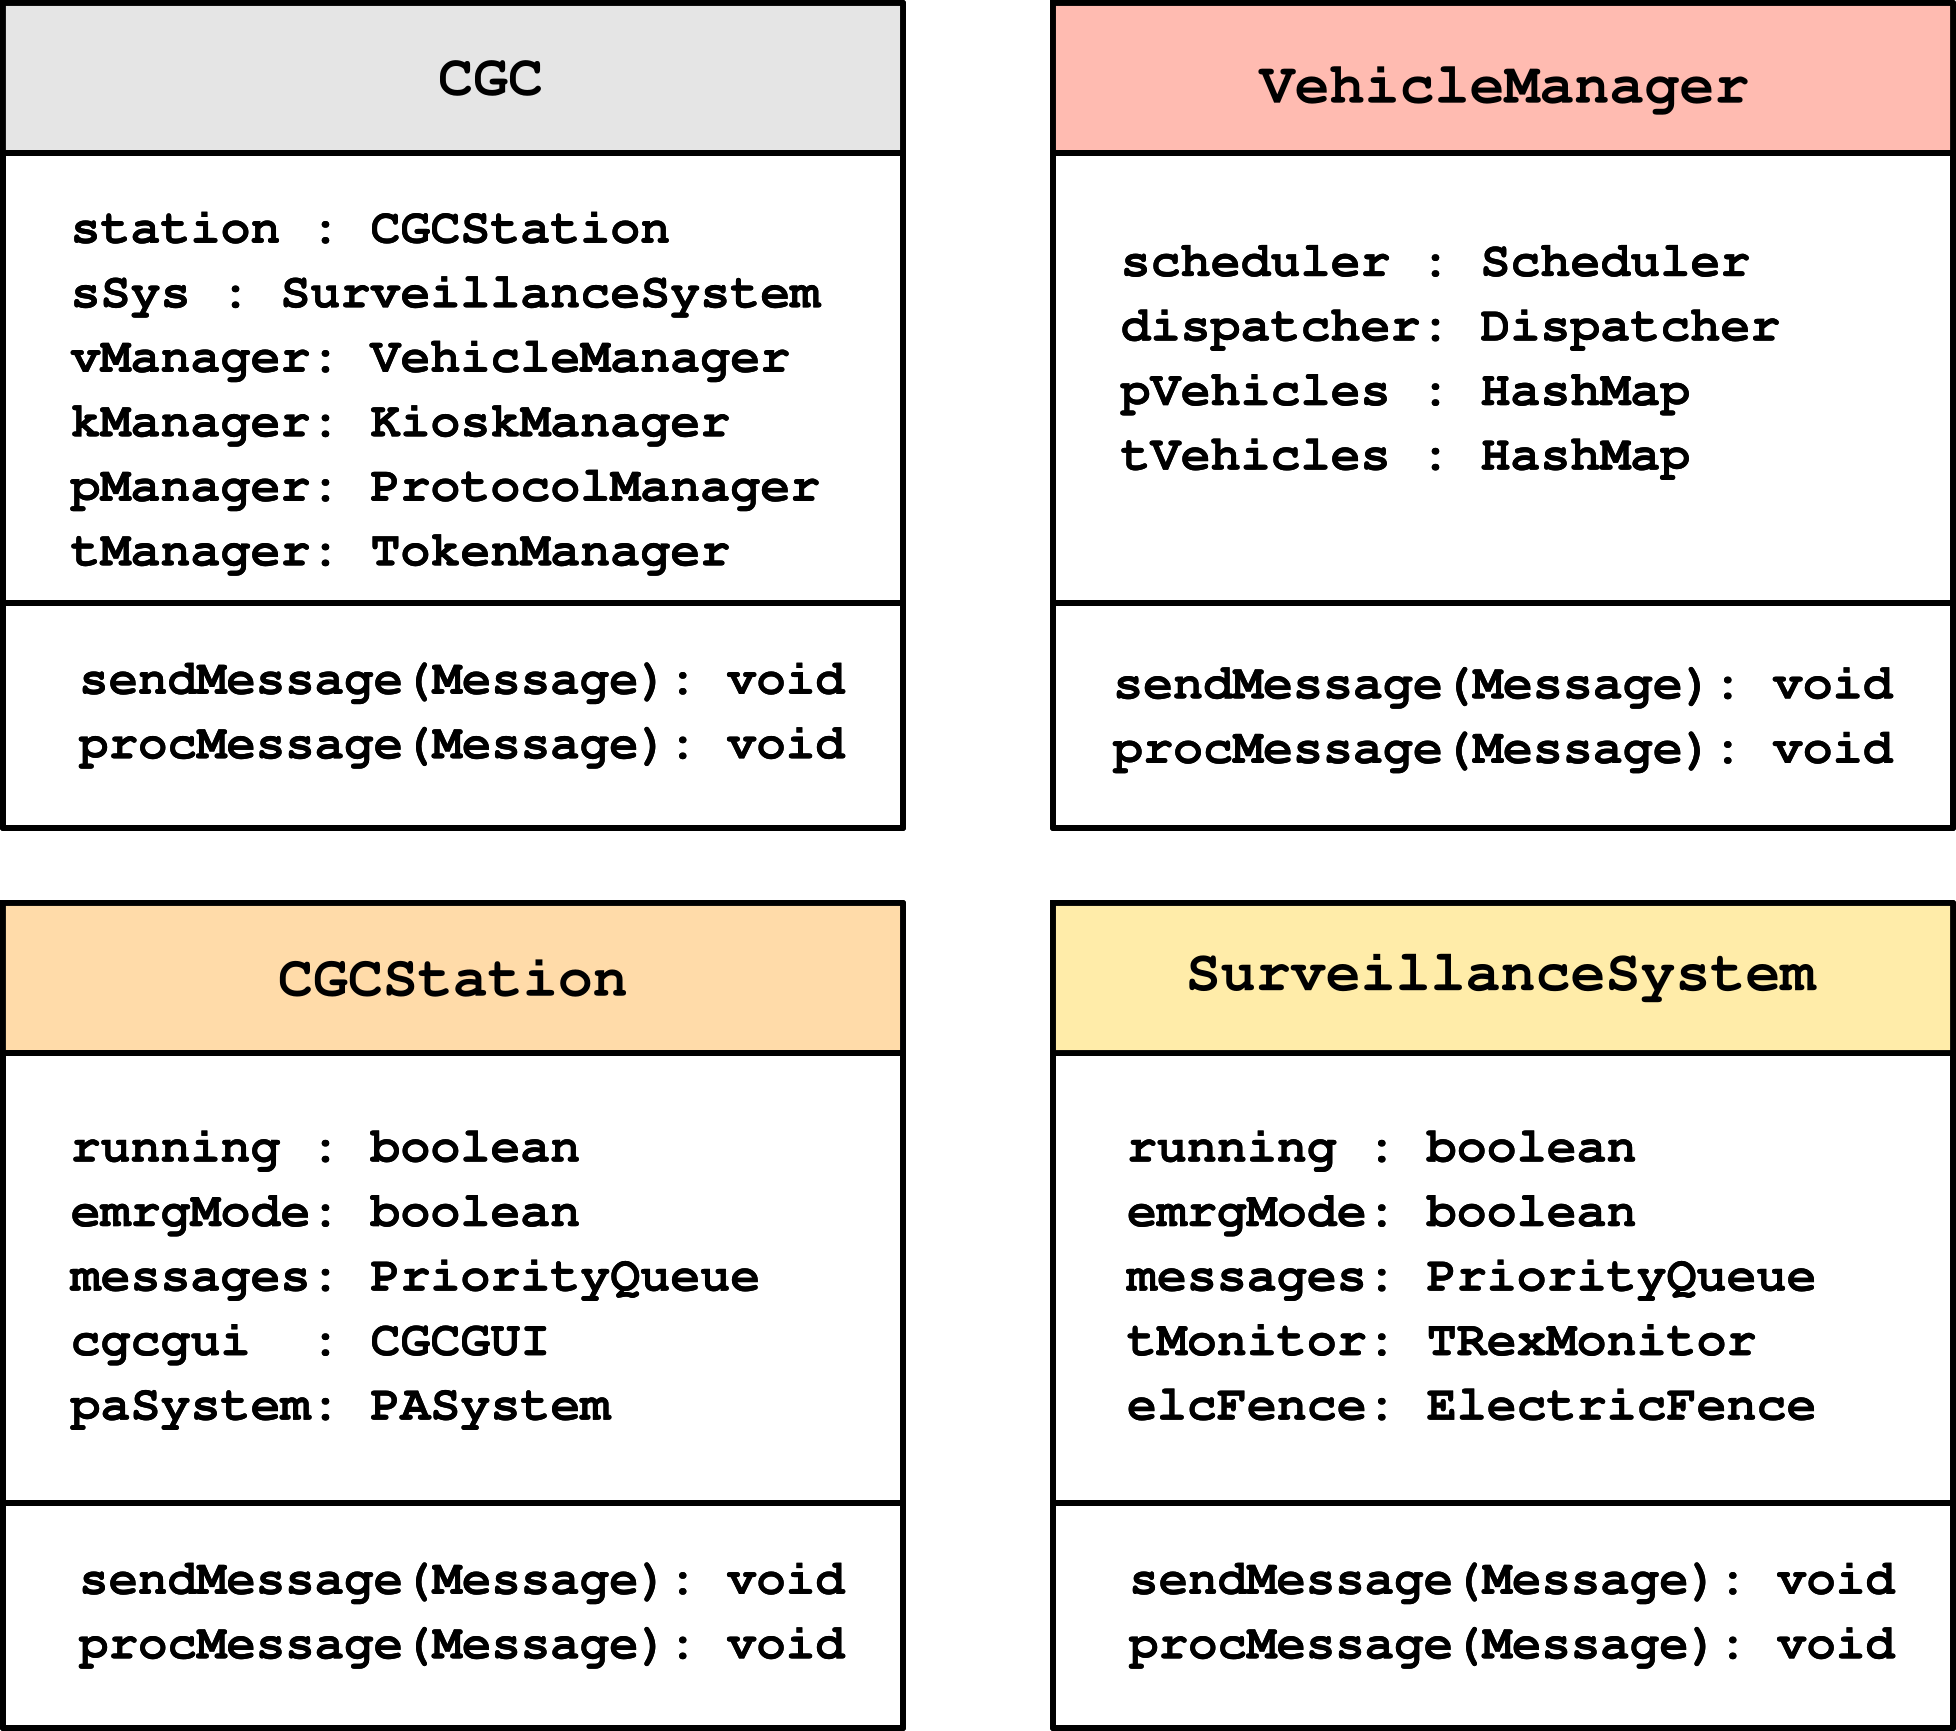
\includegraphics[scale=0.75]{MainClasses1.png}}
    \caption{\textbf{Uppermost Classes:} The \texttt{CGC} acts as a server for forwarding messages between components and
    is the parent of the others. The \texttt{VehicleManager} deals with the coordination and tracking of all vehicles, the 
    \texttt{CGCStation} is the component with which employees directly interact as it provides the visualization of the others, 
    and the \texttt{SurveillanceSystem} manages cameras and the \texttt{TRexMonitor}.}
    \label{fig:mainclasses}
\end{figure}

\begin{figure}[H]
    \centerline{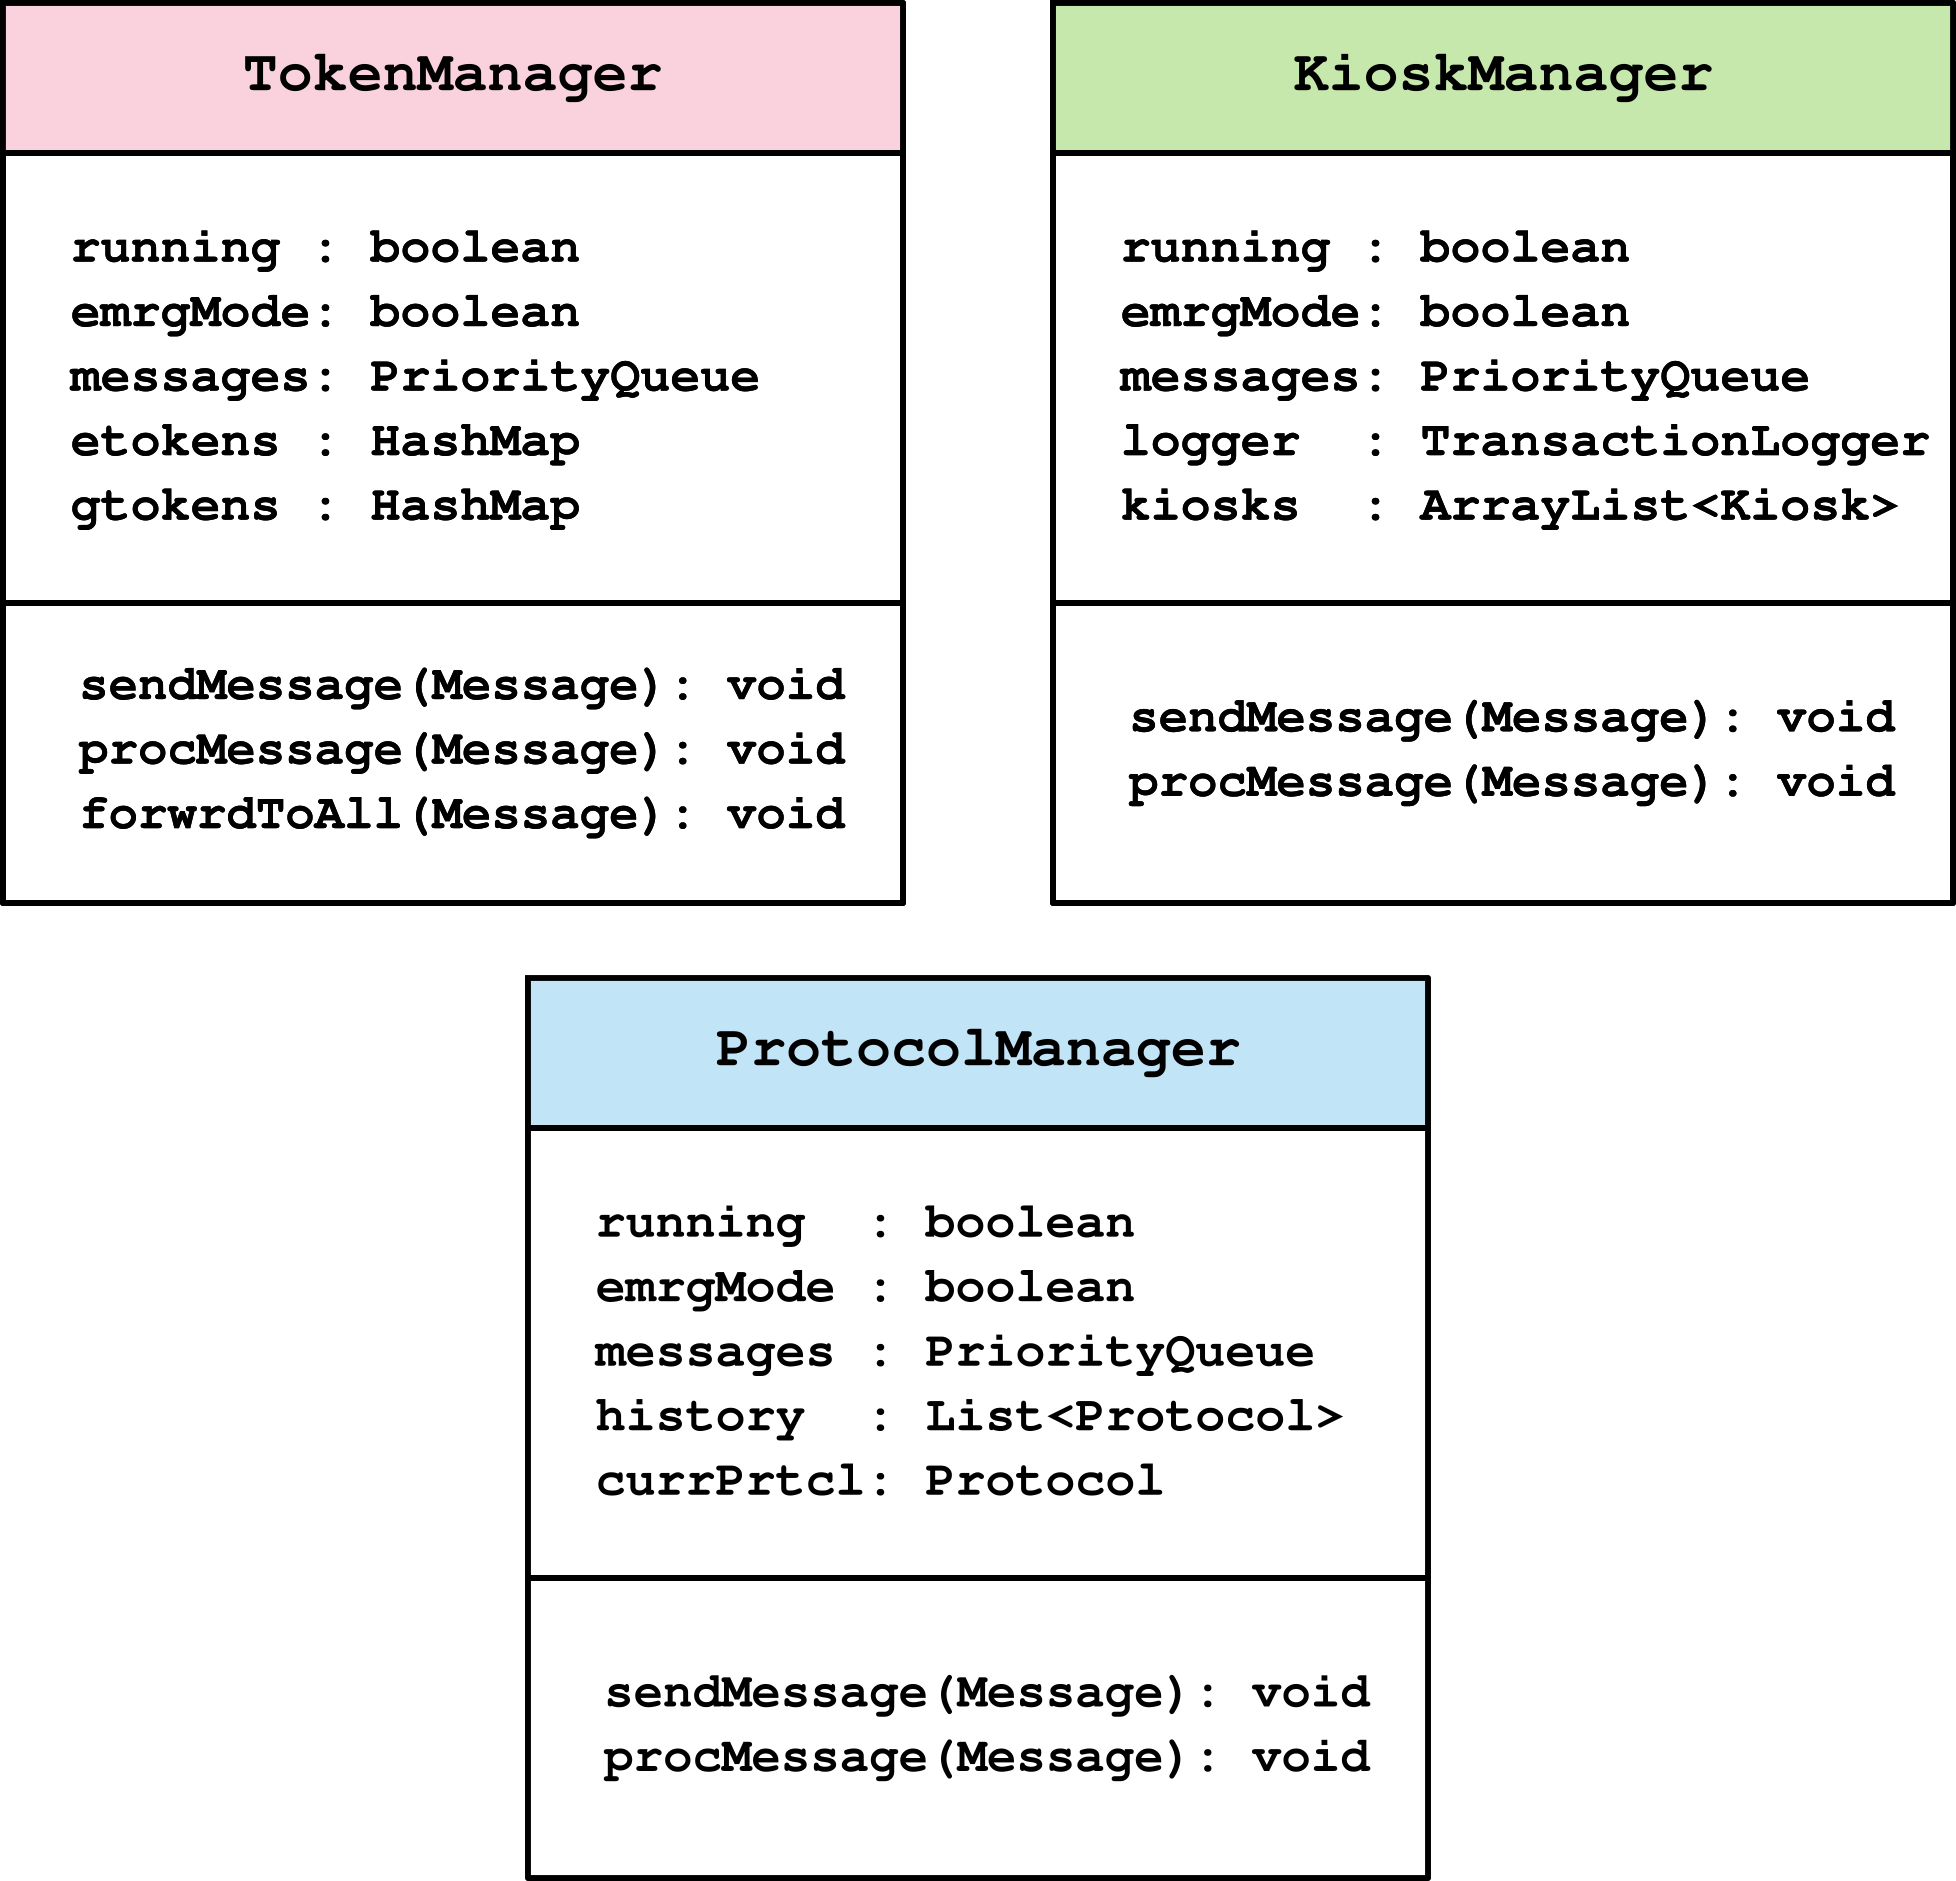
\includegraphics[scale=0.8]{MainClasses2.png}}
    \caption{\textbf{The Rest of Uppermost Classes:} The \texttt{ProtocolManager} manages the customization of protocols and maintains
    a history of which protocols have been run by the system. This component is ultimately what delivers, via the \texttt{CGC}, instructions
    on what to do in the case of an emergency. It is not implemented and its functionality is implicitly given to all components.}
    \label{fig:mainclasses2}
\end{figure}

\subsection{Vehicle Manager}
\begin{figure}[H]
    \centerline{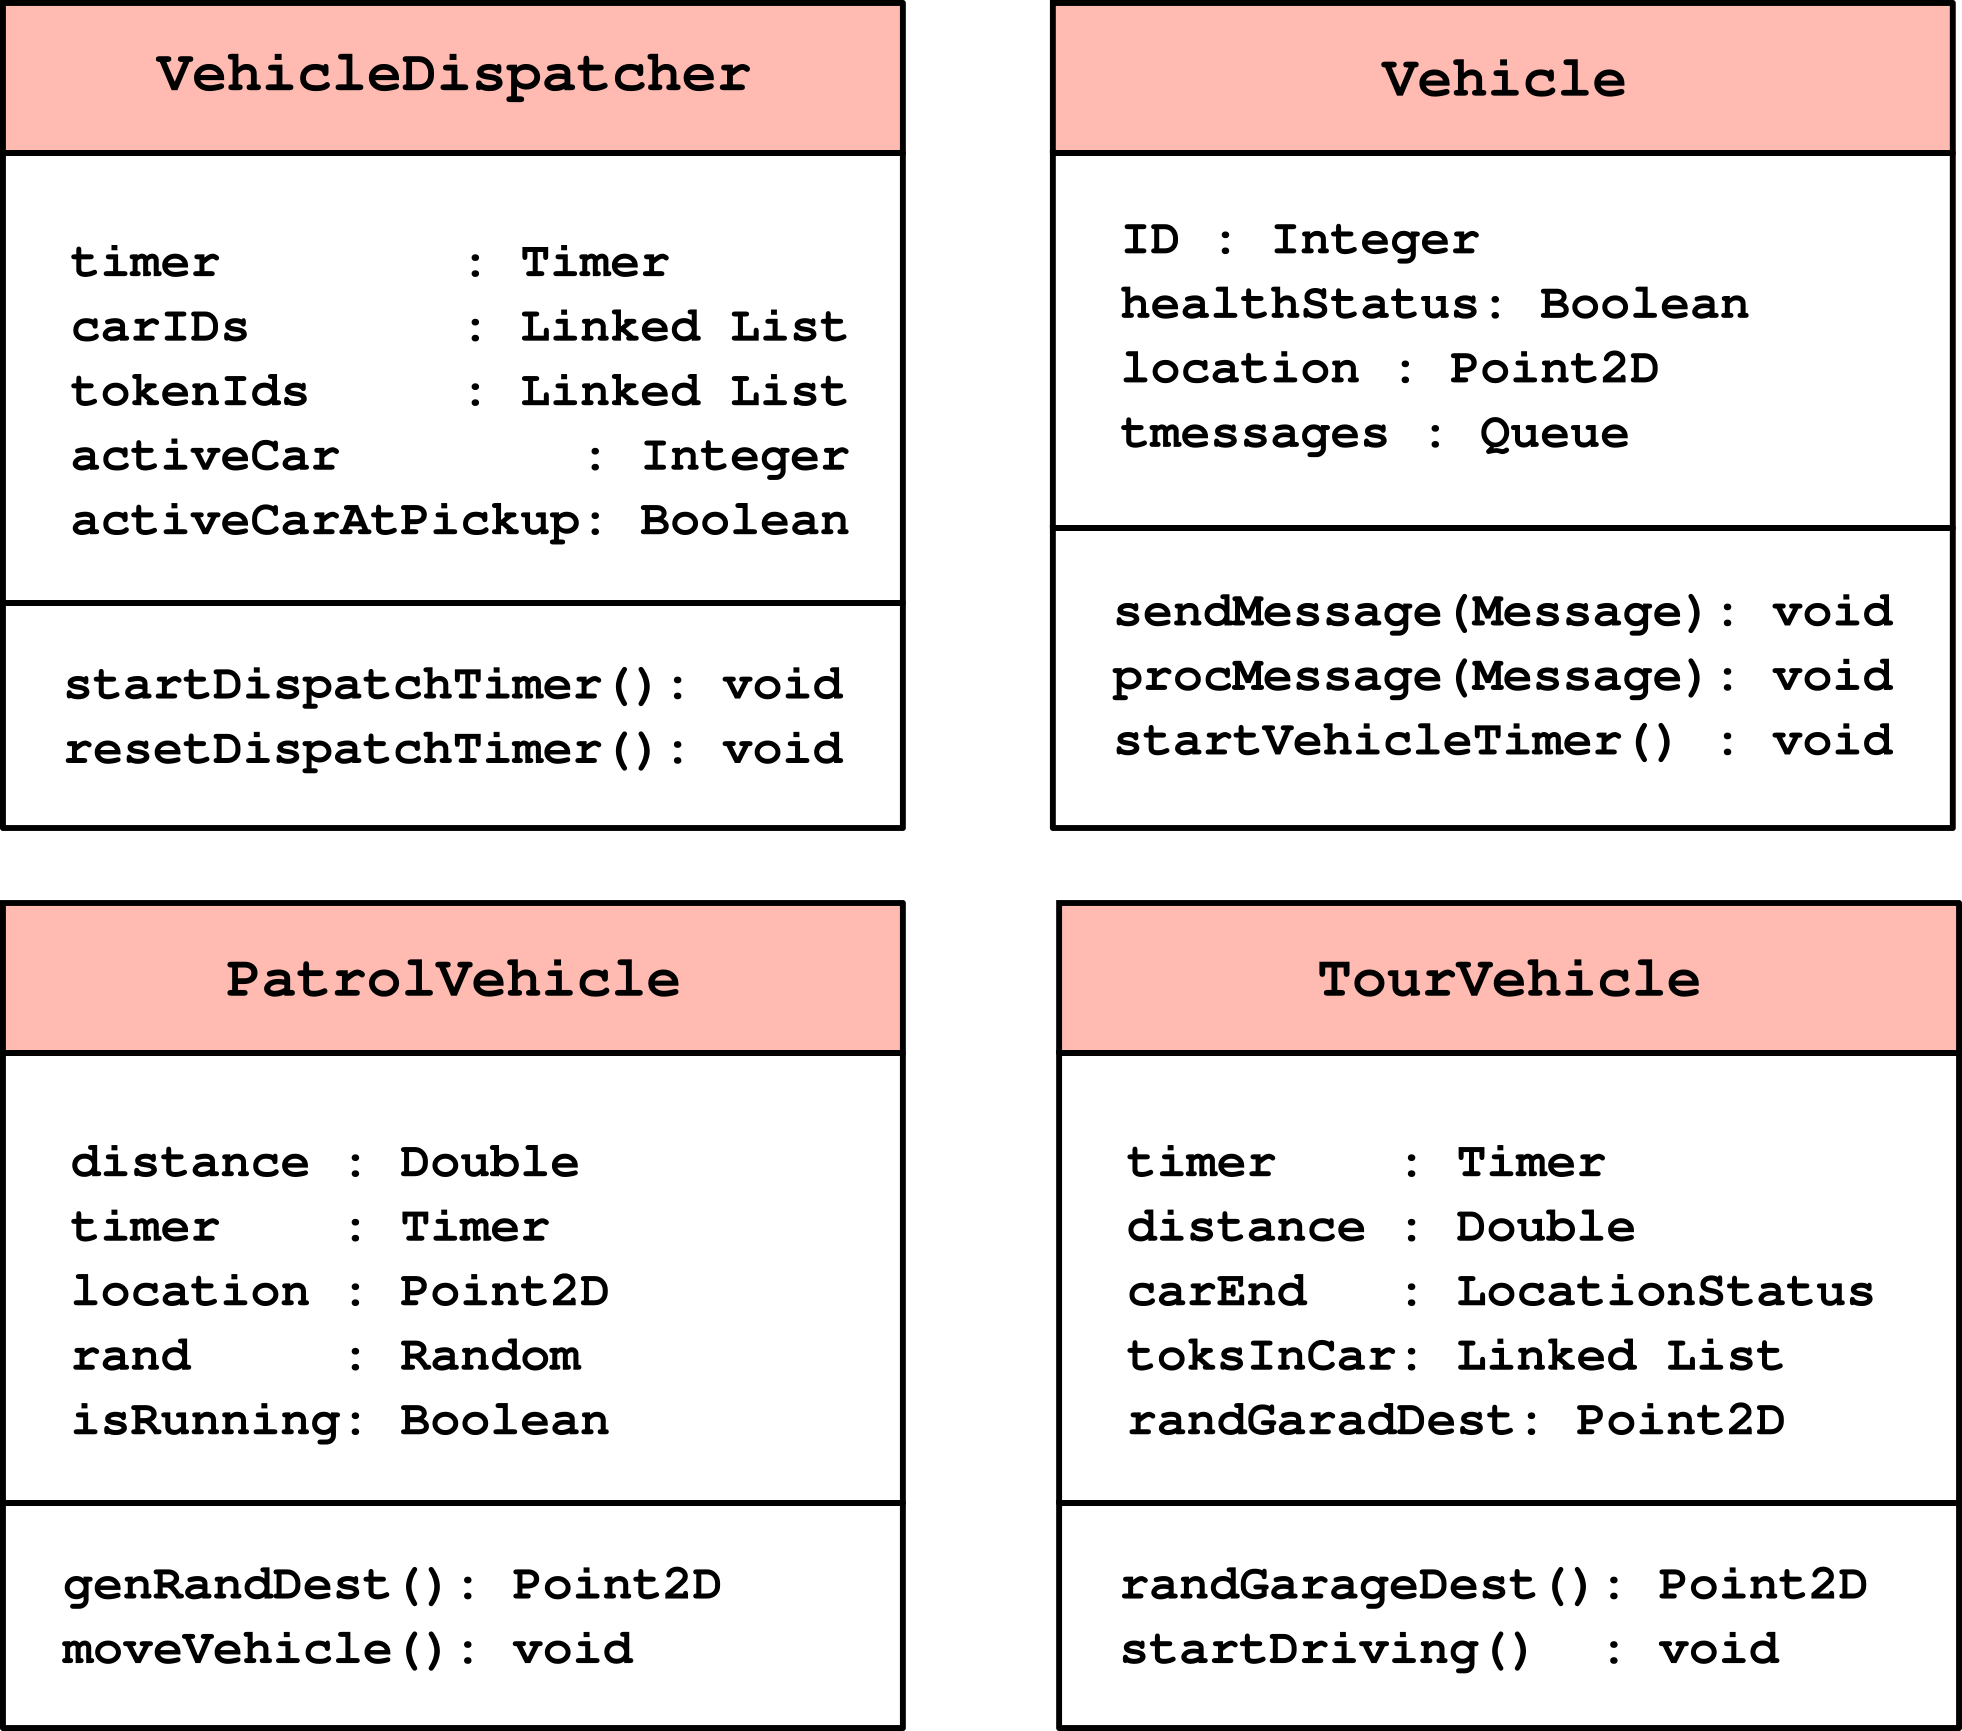
\includegraphics[scale=0.8]{VManager.png}}
    \caption{\textbf{Vehicle Manager:} The \texttt{VehicleManager} makes use of a \texttt{Dispatcher} and many \texttt{Vehicle} objects
    of which \texttt{PatrolVehicle} and \texttt{TourVehicle} are extensions.}
    \label{fig:vmanager}
\end{figure}


\subsection{CGC Station}
\begin{figure}[H]
    \centerline{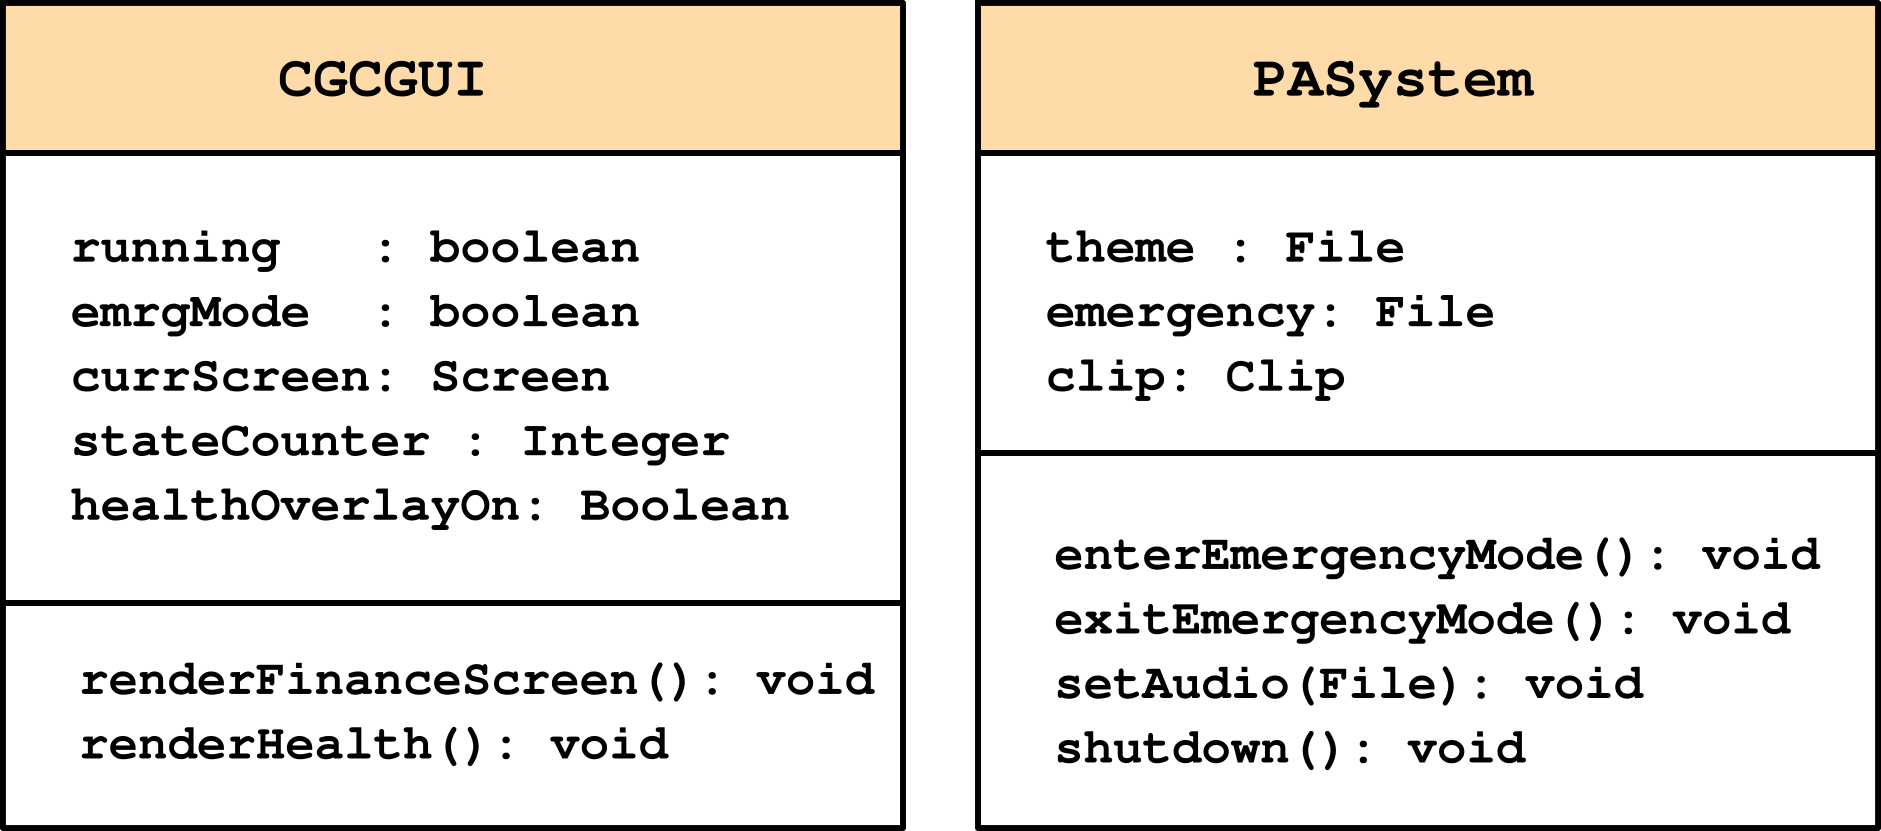
\includegraphics[scale=0.8]{CStation.png}}
    \caption{\textbf{CGC Station:} The \texttt{CGCStation} makes use of a \texttt{CGCGUI} and a \texttt{PASystem} object.
    The first shows graphical representations of the system for an employee, and the second encapsulates the central 
    communication module for the island.}
    \label{fig:cstation}
\end{figure}

\subsection{Surveillance System}
\begin{figure}[H]
    \centerline{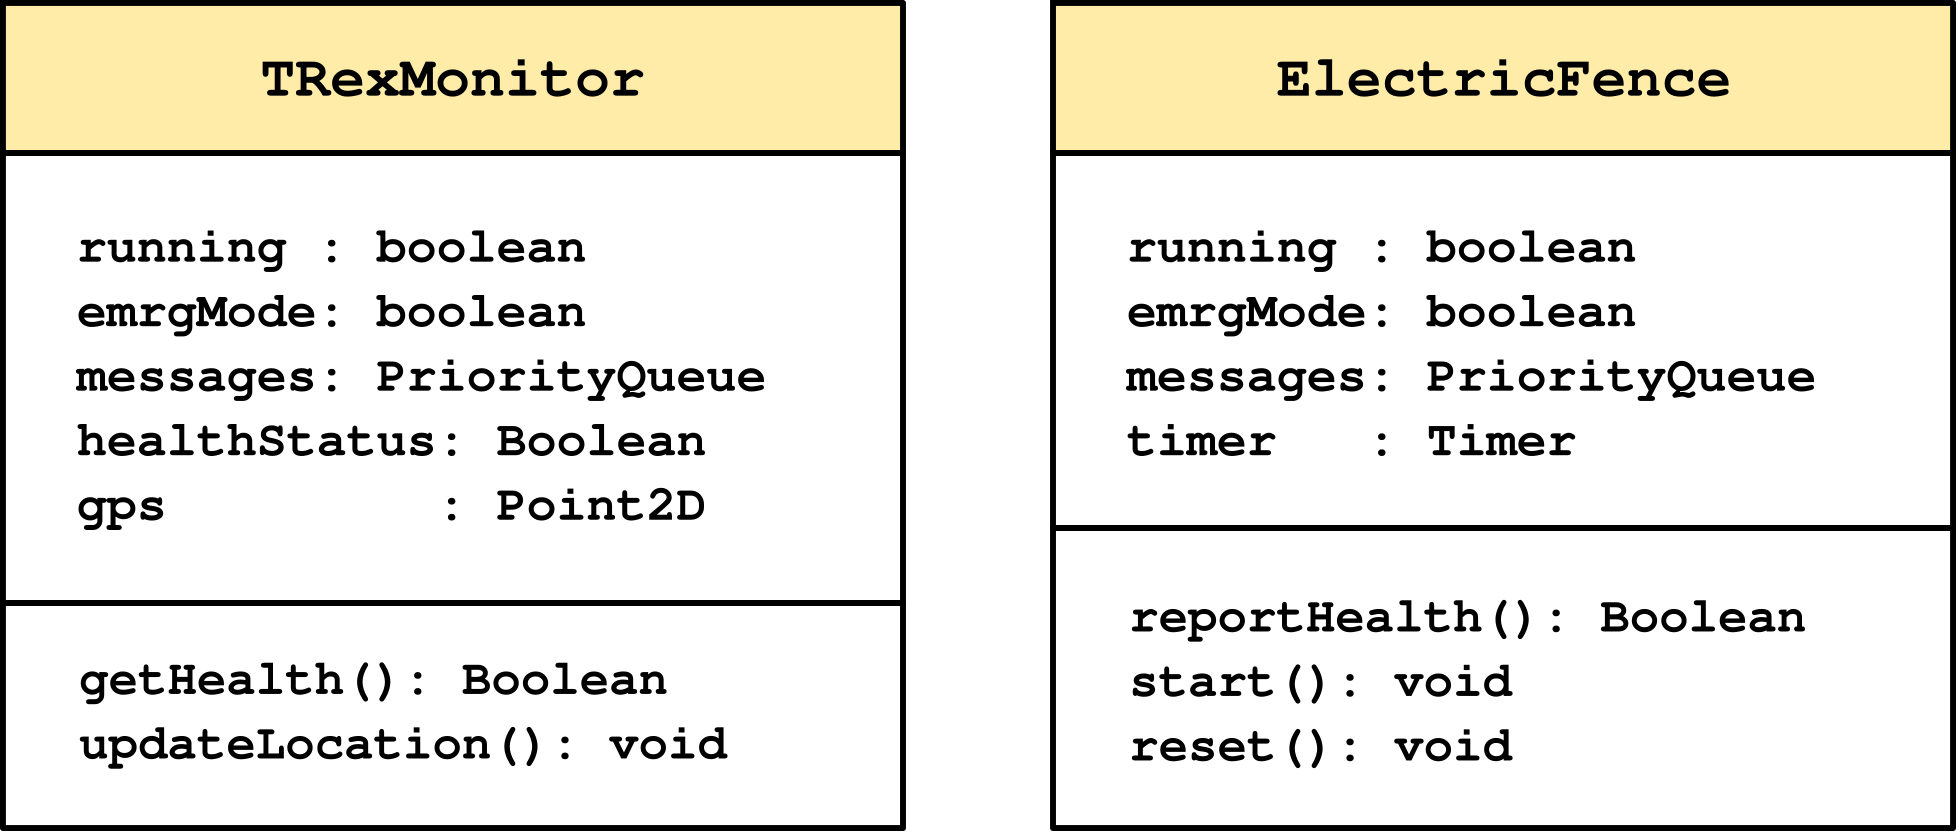
\includegraphics[scale=0.8]{SSystem.png}}
    \caption{\textbf{Surveillance System:} The \texttt{SurveillanceSystem} makes use of a \texttt{TRexMonitor} and an 
    \texttt{ElectricFence} object.}
    \label{fig:ssystem}
\end{figure}

\subsection{Token Manager}
\begin{figure}[H]
    \centerline{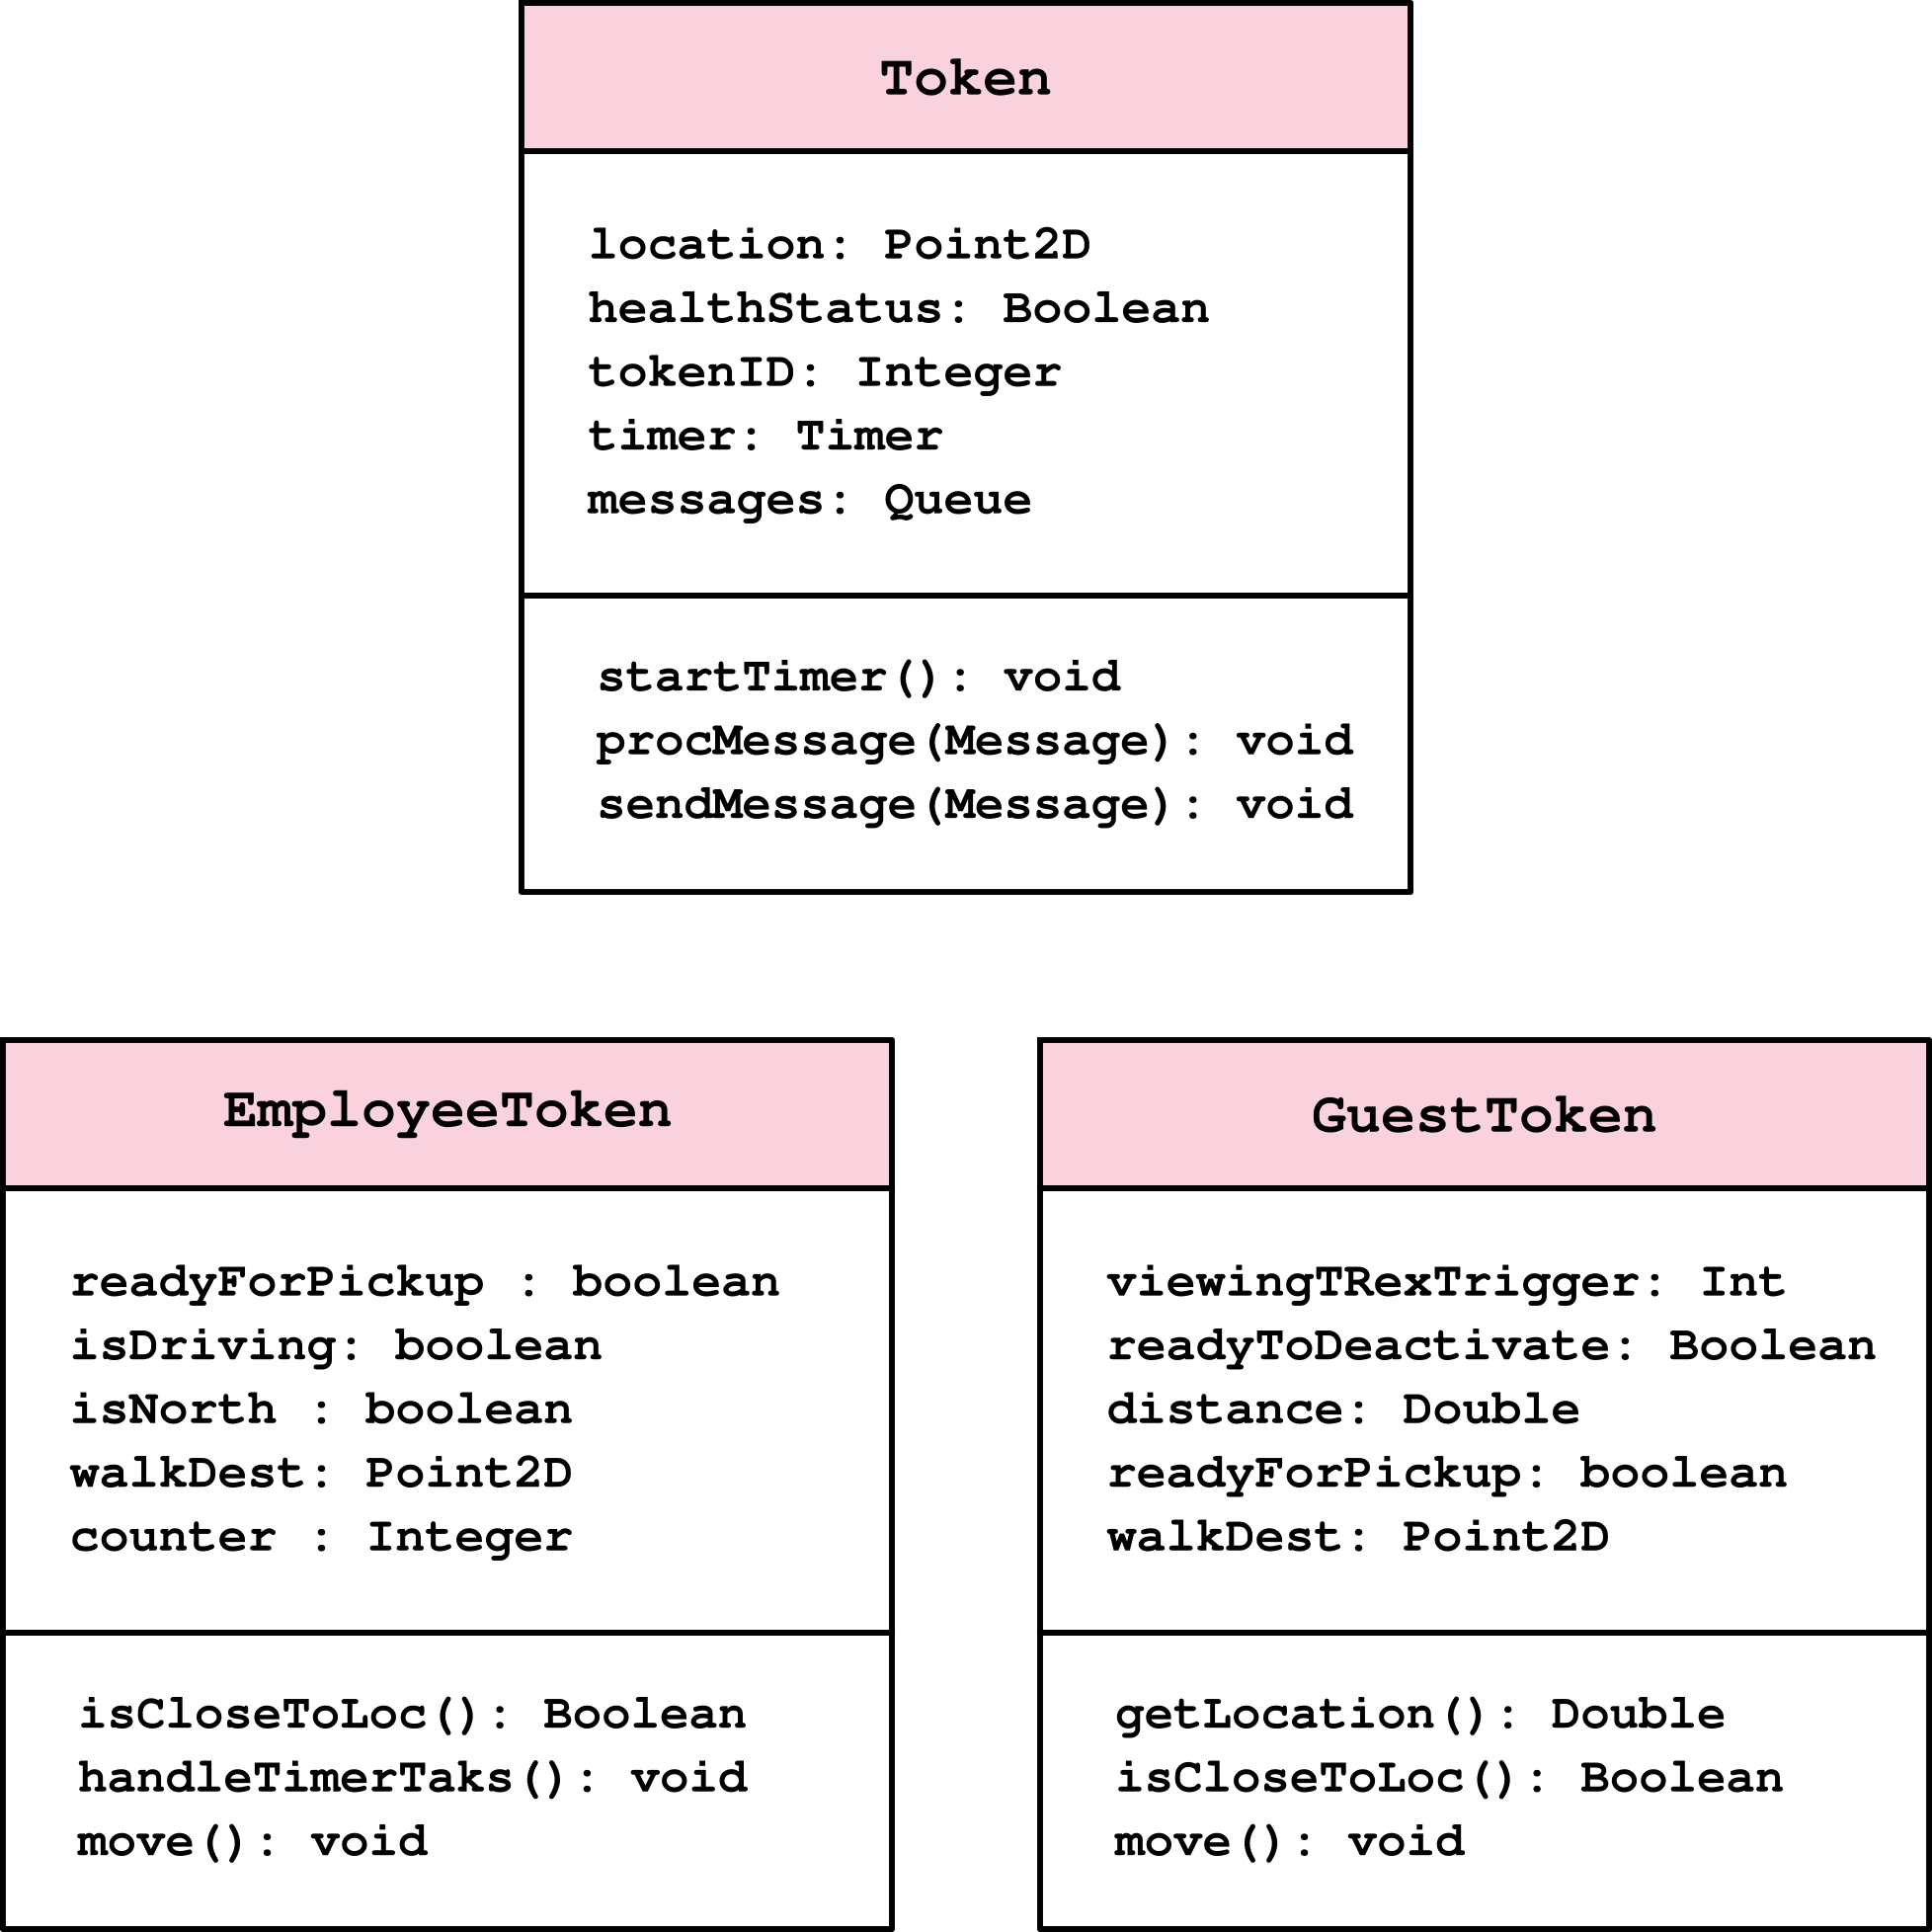
\includegraphics[scale=0.8]{TManager.png}}
    \caption{\textbf{Token Manager:} The \texttt{TokenManager} makes use of \texttt{Token} objects
    of which \texttt{GuestToken} and \texttt{EmployeeToken} are extensions.}
    \label{fig:tmanager}
\end{figure}


\subsection{Kiosk Manager}
\begin{figure}[H]
    \centerline{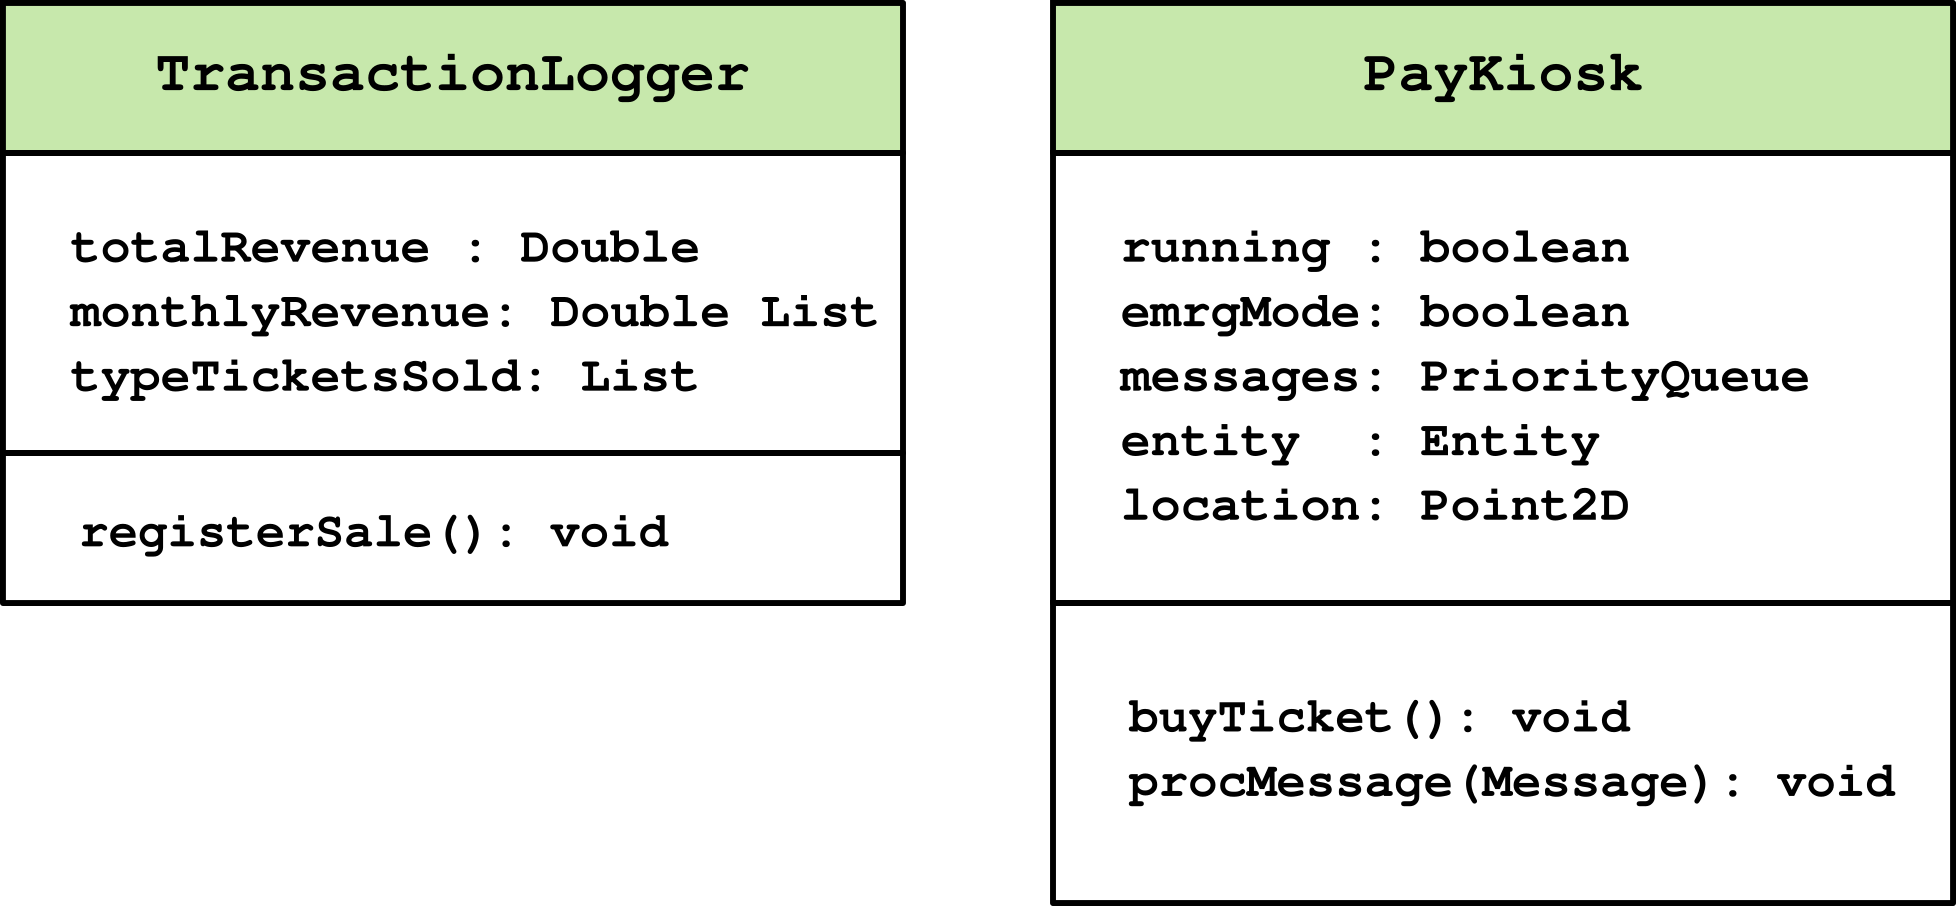
\includegraphics[scale=0.8]{KManager.png}}
    \caption{\textbf{Kiosk Manager:} The \texttt{} makes use of a \texttt{} and many \texttt{} objects
    of which \texttt{} and \texttt{} are extensions.}
    \label{fig:kmanager}
\end{figure}


\section{Sample Use Cases} \label{samp}
\paragraph{} \textit{A broad overview of use cases begins this section and it is followed 
by detailed case descriptions. Human actors are denoted by small stick figures and have the 
same color scheme as the box that contains their labels. This section has been generalized into
three types of users for simplicity. Guests, internal personnel, and external personnel constitute
the types of actors. Guests are park visitors, internal personnel are those actors that contribute 
(typically through daily employment) to the function of the resort on a regular basis (e.g. cars, 
maintenance personnel, the T.Rex), and external personnel are actors which interact with the system
on an irregular or infrequent basis (e.g. veterinarians, auditors, emergency personnel).}

\pagebreak
\subsection{Guests}
\begin{figure}[H]
    \centerline{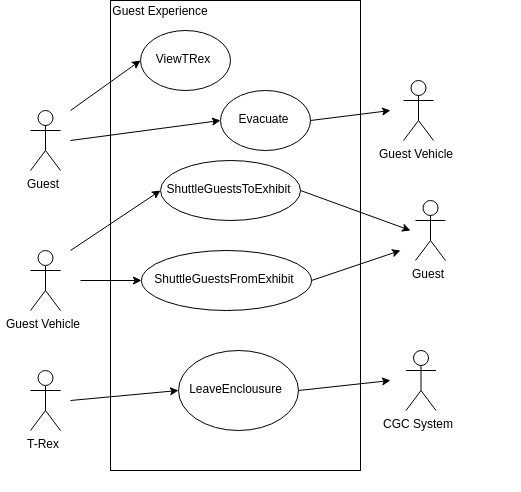
\includegraphics[scale=.30]{Use_Cases__Guest.png}}
    \caption{Shows the a general view of the Guest Use Case as a diagram.}
    \label{fig:usecaseguest}
\end{figure}
\small
    \begin{itemize}
        \item[]\textbf{Use Case:}                                
            ViewTRex

        \item[]\textbf{Primary Actor:}
            Guest

        \item[]\textbf{Goal in Context:}
            To see a live dinosaur.

        \item[]\textbf{Preconditions:}
            The system and all components are functioning normally.
            
        \item[]\textbf{Trigger:}
            The guest wishes to see a dinosaur since the age of five.

        \item[]\textbf{Scenario:}
            \begin{enumerate}
                \item Upon hearing of the grand opening of Cretaceous Gardens, the guest immediately
                heads to the island by whatever means possible.
                \item On arrival, the guest witnesses tremendous lines formed at many pay kiosks
                near the entrance of the resort.
                \item After what seems like an eternity, the it is the guest's turn to purchase entry to the resort.
                \item The guest is welcomed through a pleasant graphical display.
                \item The guest is asked a series of questions in order verify compliance with the park policies
                (e.g. How old are you? Do you consent to having your picture taken? Do you accept full responsibility 
                for any injuries sustained due to personal choices? Do you accept the risks of seeing a live 
                Tyrannosaurus Rex and free Cretaceous Gardens of any and all consequences of doing so?)
                \item After ignoring all the fine print and zipping through the legal stuff, the guest finally
                arrives at the screen that will allow the rental of an access token.
                \item The guest enters the amount of time he or she plans to stay and is given the total price.
                \item The guest is prompted to enter payment.
                \item The guest pays after confirmation and receives the rental token device.
                \item Instructions on what to do next are displayed on the kiosk screen.
                \item The guest uses the token device to enter the resort via a small gate.
                \item The guest eventually arrives at a parked car, into which others may or may not be entering.
                \item The guest enters the token device into the seatbelt buckle and secures the seatbelt.
                \item The guest lets the car do its job (see section \ref{carscenarios}).
                \item The guest arrives at the exhibit and exits the car, taking the token device along.
                \item The guest heads toward another gate which scans the token device to provide access.
                \item The guest sprints toward the enclosure.
                \item The guest is lucky and gets to see the mighty T.Rex sniffing around. 
            \end{enumerate}

        \item[]\textbf{Exceptions:}
            \begin{itemize}
                \item[] Guest changes his or her mind anywhere in the scenario and decides to leave.
                \item[] The system is triggered into emergency mode.
            \end{itemize}

        \item[]\textbf{Priority:}
            Essential, must be implemented.

        \item[]\textbf{When Available:}
            On Demand.

        \item[]\textbf{Frequency of Use:}
            Up to thousands of times per day.

        \item[]\textbf{Channel to Primary Actor:}
            Direct.

        \item[]\textbf{Channels to Secondary Actors:}
            \begin{itemize}
                \item[] Kiosk: Display on kiosk.
                \item[] Token: Device display and speaker.
                \item[] Guest Vehicle: Token interfaces and seat sensors.
                \item[] T-Rex: Seen through enclosure fence.
            \end{itemize}
        \item[]\textbf{Secondary Actors:}
            Kiosk, Token, Guest Vehicle, T-Rex.

        \item[]\textbf{Open Issues:}
            None known.
    \end{itemize}

    \par\noindent\rule{\textwidth}{0.4pt}    
    \begin{itemize}
        \item[]\textbf{Use Case:}                                
            Evacuate

        \item[]\textbf{Primary Actor:}
            Guest

        \item[]\textbf{Goal in Context:}
            To leave the island as quickly and as safely as possible.

        \item[]\textbf{Preconditions:}
            There exists some imminent threat to the guest (it may be an enclosure failure, inclement 
            weather, or any other emergency of similar caliber). Sudden guest death (unrelated to the
            island or system) may also be the case.

        \item[]\textbf{Trigger:}
            Something horrible occurs. For simplicity, the following scenario assumes the T-Rex destroys
            its enclosure and is now on the loose.

        \item[]\textbf{Scenario:}
            \begin{enumerate}
                \item The T-Rex destroys the enclosure (see subsection \ref{trexleave}).
                \item Emergency mode is activated.
                \item22 All guests are alerted via the car intercom, the token devices, and an
                island wide speaker system, the Global Alarm System.
                \item Guests receive instructions via the above means with interleaved reassurances
                that extra vehicles are on the way to pick them up.
                \item Guests are also informed that they may enter any vehicle, with or without tokens.
                \item Once in the vehicle, guests are asked (via the token device) whether or not
                they would like to depart.
                \item If at least one individual submits a yes, the car transmits a message to indicate
                imminent departure with a warning that doors will soon close.
                \item Once in motion, the guest in the driver seat is offered the option to place the vehicle into
                manual mode.
                \item If the individual chooses to do so, then he or she may now pilot the vehicle as he or she wishes.
                \item Otherwise, the car will head south as quickly and as safely as possible.
                \item Once at the south end, the car will park and wait for guests to exit.
                \item After it has been confirmed that no guests remain in the vehicle (seat weight sensors
                indicate all seats are empty), the guests are given another warning to stand back.
                \item As the guests head toward the exit, the car closes its doors and speeds north 
                to collect more guests.
            \end{enumerate}

        \item[]\textbf{Exceptions:}
            \begin{itemize}
                \item[] The car suffers damage that causes it to malfunction.
            \end{itemize}

        \item[]\textbf{Priority:}
            Essential, must be implemented.

        \item[]\textbf{When Available:}
            On demand.

        \item[]\textbf{Frequency of Use:}
            Hopefully never, but at least once in reality.

        \item[]\textbf{Channel to Primary Actor:}
            Car doors, tokens, interior car components (if manual mode is enabled)
            
        \item[]\textbf{Channels to Secondary Actors:}
            \begin{itemize}
                \item[] T-Rex: breached enclosure
                \item[] Token: device display and speaker
                \item[] Emergency Personnel: directly at any stage during the evacuation.
            \end{itemize}
        \item[]\textbf{Secondary Actors:}
            T.Rex, Tokens, Emergency Personnel

        \item[]\textbf{Open Issues:}
            \begin{itemize}
                \item[] None known.
            \end{itemize}
    \end{itemize}

\subsection{Internal Personnel}
\begin{figure}[H]
    \centerline{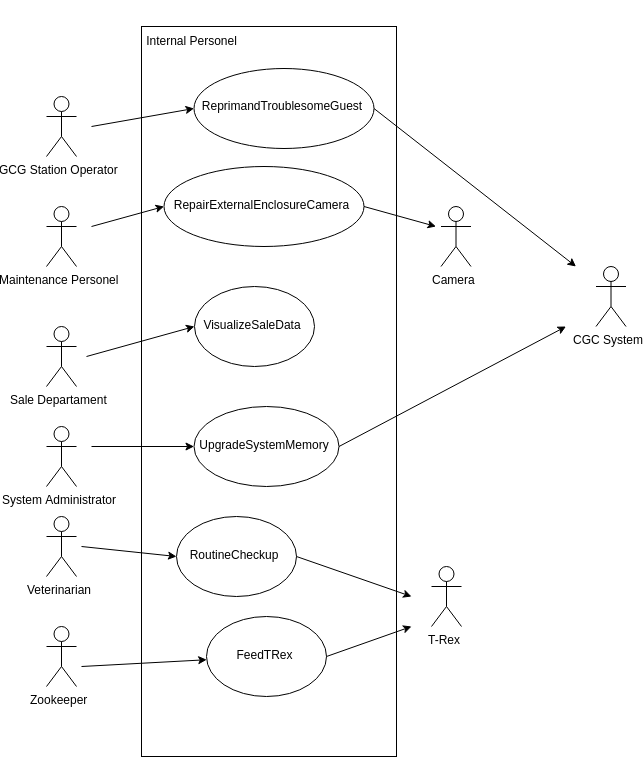
\includegraphics[scale=.30]{Use_Cases__Internal.png}}
    \caption{Shows the a general view of the Internal Personnel Use Cases as a diagram.}
    \label{fig:usecaseinternal}
\end{figure}    
    \begin{itemize}
        \item[]\textbf{Use Case:}                                
            ReprimandTroublesomeGuest

        \item[]\textbf{Primary Actor:}
            CGC Station Operator

        \item[]\textbf{Goal in Context:}
            To reprimand a guest that is causing trouble by incremental warnings ranging from
            casual notice, to threats of banishment from the resort.

        \item[]\textbf{Preconditions:}
            The system and all components are functioning properly.

        \item[]\textbf{Trigger:}
            A guest is caught throwing rocks into the enclosure.
            
        \item[]\textbf{Scenario:}
            \begin{enumerate}
                \item The GSO reviews an alert from the electric fence interface.
                \item The GSO reads that small voltage spikes have been detected.
                \item The GSO heads to the surveillance camera that corresponds to the
                panel in question.
                \item The GSO observes a guest hurling rocks at the enclosure, which
                explains the voltage spikes.
                \item The GSO immediately and firmly tells the guest to stop throwing rocks
                through the PA system near the site.
                \item The GSO is ignored by the guest who gives the finger to the camera.
                \item The GSO dispatches the nearest patrol vehicle to the location.
                \item The GSO explains the situation to the security guard that happens 
                to be in the patrol vehicle at the time.
                \item The GSO firmly alerts the unruly guest that a security guard has been sent.
                \item The security guard arrives and reprimands the guest.
                \item The guest become violent and gets tased and pepper sprayed.
                \item The guest is apprehended and placed in the patrol vehicle.
                \item The GSO dismisses the electric fence alerts.
            \end{enumerate}

        \item[]\textbf{Exceptions:}
            \begin{itemize}
                \item[] The system is triggered into emergency mode.
            \end{itemize}

        \item[]\textbf{Priority:}
            Moderate, not necessary, but can be useful.
            
        \item[]\textbf{When Available:}
            On demand.

        \item[]\textbf{Frequency of Use:}
            More frequent with higher volumes of visits.
            
        \item[]\textbf{Channel to Primary Actor:}
            Electric fence panel, CGC Station GUI, camera 

        \item[]\textbf{Secondary Actors:}
            Patrol Vehicle, Security Guard, Electric Fence, Guest
            
        \item[]\textbf{Channels to Secondary Actors:}
            \begin{itemize}
                \item[] Patrol Vehicle: direct
                \item[] Security Guard: car intercom
                \item[] Electric Fence: direct
                \item[] Guest: PA system, electric fence
            \end{itemize}

        \item[]\textbf{Open Issues:}
            \begin{itemize}
                \item[] None known.
            \end{itemize}
    \end{itemize}
    
    \par\noindent\rule{\textwidth}{0.4pt}    
    \begin{itemize}
        \item[]\textbf{Use Case:}                                
            ShuttleGuestsToExhibit

        \item[]\textbf{Primary Actor:}
            Guest Vehicle

        \item[]\textbf{Goal in Context:}
            To transport guests to the northern part of the island so they may 
            visit the exhibit.

        \item[]\textbf{Preconditions:}
            The system is in normal mode and all components are functioning properly.

        \item[]\textbf{Trigger:}
            A transaction is confirmed and a tokens are provided to guests.

        \item[]\textbf{Scenario:}
            \begin{enumerate}
                \item The guests are directed to the parked GV.
                \item The guests enter the GV.
                \item The GV instructs guests to enter their token devices into their belt buckles.
                \item The GV detects all token-containing buckles have been used to fasten corresponding seatbelts.
                \item The GV locks its doors and unlocks window functionality for guests.
                \item The GV performs a quick system check.
                \item The GV heads toward the exhibit.
                \item The GV arrives and parks in front of a gate that leads to the exhibit.
                \item The GV reminds the guests to take their tokens with them as it grants them access through the gate.
                \item The guests exit the vehicle and make their way toward the gate.
                \item The GV parks itself nearby and starts a timer.
            \end{enumerate}

        \item[]\textbf{Exceptions:}
            \begin{itemize}
                \item[] A guest loses his or her token device, thus preventing seatbelt access, which necessitates
                staff intervention.
            \end{itemize}

        \item[]\textbf{Priority:}
            Essential, must be implemented.

        \item[]\textbf{When Available:}
            On Demand.

        \item[]\textbf{Frequency of Use:}
            Up to thousands of times per day.
            
        \item[]\textbf{Channel to Primary Actor:}
            Direct.

        \item[]\textbf{Secondary Actors:}
            Guests, CGC Station Operator, Tokens
            
        \item[]\textbf{Channels to Secondary Actors:}
            \begin{itemize}
                \item[] Guests: doors, seatbelts, speakers
                \item[] CGC Station Operator: direct
                \item[] Tokens: seatbelt buckles
            \end{itemize}

        \item[]\textbf{Open Issues:}
            \begin{itemize}
                \item[] None known.
            \end{itemize}
    \end{itemize}

    \par\noindent\rule{\textwidth}{0.4pt}    
    \begin{itemize}
        \item[]\textbf{Use Case:}                                
            ShuttleGuestsFromExhibit

        \item[]\textbf{Primary Actor:}
            Guest Vehicle

        \item[]\textbf{Goal in Context:}
            To transport guests to the southern part of the island so they may 
            leave the island.

        \item[]\textbf{Preconditions:}
            The system is in normal mode and all components are functioning properly.

        \item[]\textbf{Trigger:}
            The guests' time is up at the exhibit.

        \item[]\textbf{Scenario:}
            \begin{enumerate}
                \item The car alerts the guests it shuttled to the exhibit that time is up.
                \item The guests hear the alert from the car and from their token devices.
                \item Some of the guests immediately head to the car while others delay.
                \item The guests that head to the car enter it and fasten their seat belts.
                \item The GV sends another alert to those remaining.
                \item The rest of the guests finally arrive and enter the GV.
                \item The GV locks its doors after everyone has fastened their seatbelts.
                \item The GV heads south.
                \item The GV arrives to the southern part of the island where it parks.
                \item The guests release their seatbelts.
                \item The GV unlocks its doors and allows the guests to exit.
                \item The GV is dispatched elsewhere.
            \end{enumerate}

        \item[]\textbf{Exceptions:}
            \begin{itemize}
                \item[] A guest happens to be injured and requires another type of transportation.
                \item[] A guest loses his or her token device, thus preventing seatbelt access.
            \end{itemize}

        \item[]\textbf{Priority:}
            Essential, must be implemented.

        \item[]\textbf{When Available:}
            On Demand.

        \item[]\textbf{Frequency of Use:}
            Up to thousands of times per day.
            
        \item[]\textbf{Channel to Primary Actor:}
            Direct.

        \item[]\textbf{Secondary Actors:}
            Guests, CGC Station Operator, Tokens
            
        \item[]\textbf{Channels to Secondary Actors:}
            \begin{itemize}
                \item[] Guests: doors, seatbelts, speakers
                \item[] CGC Station Operator: direct
                \item[] Tokens: seatbelt buckles
            \end{itemize}

        \item[]\textbf{Open Issues:}
            \begin{itemize}
                \item[] None known.
            \end{itemize}
    \end{itemize}
    
    \par\noindent\rule{\textwidth}{0.4pt}    
    \begin{itemize}
        \item[]\textbf{Use Case:} 
            FeedTRex                                

        \item[]\textbf{Primary Actor:}
            Zookeeper

        \item[]\textbf{Goal in Context:}
            To safely provide food for the T.Rex, whether it be live, frozen, thawed, or prepared
            prey.

        \item[]\textbf{Preconditions:}
            The CGC is not in emergency mode, and all components are fully functional.

        \item[]\textbf{Trigger:}
            It is time to feed the T.Rex.

        \item[]\textbf{Scenario:}
            \begin{enumerate}
                \item The CGC Station Operator dispatches the zookeeper in a self driving car
                to the edge of the enclosure furthest from the current location of the T.Rex.
                \item The Zookeeper requests an all-clear confirmation from the operator.
                \item The operator disengages the electricity of the panel to provide access.
                \item The Zookeeper enters and travels a significant distance into the enclosure.
                \item The Zookeeper drops off the food.
                \item The Zookeeper travels back the point of entry.
                \item The Zookeeper exits the enclosure.
                \item The Operator confirms successful exit.
                \item The Operator reengages the electricity of the panel. 
            \end{enumerate}

        \item[]\textbf{Exceptions:}
            \begin{itemize}
                \item[] There is a shortage of food on the island.
                \item[] The T.Rex is sick or injured and does not want to eat.
                \item[] The T.Rex reaches the zookeeper before the zookeeper exits the enclosure.
            \end{itemize}

        \item[]\textbf{Priority:}
            Essential, must be implemented

        \item[]\textbf{When Available:}
            On demand and via operator-zookeeper protocol

        \item[]\textbf{Frequency of Use:}
            Periodically (it can be daily, weekly, or monthly for example)

        \item[]\textbf{Channel to Primary Actor:}
            \begin{itemize}
                \item[] Enclosure Panel
            \end{itemize}

        \item[]\textbf{Secondary Actors:}
            CGC Station Operator, T.Rex, Car
        
        \item[]\textbf{Channels to Secondary Actors:}
            \begin{itemize}
                \item[] CGC Station Operator: Car Intercom, Camera Network
                \item[] T.Rex: Enclosure Panel
            \end{itemize}

        \item[]\textbf{Open Issues:}
            \begin{itemize}
                \item[] Should the panel remain inactive while 
                the zookeeper is inside?
                \item[] Should the zookeeper simply wear an electric 
                safety suit to avoid disengagement all together?
            \end{itemize}
    \end{itemize}

\subsection{External Personnel}
\begin{figure}[H]
    \centerline{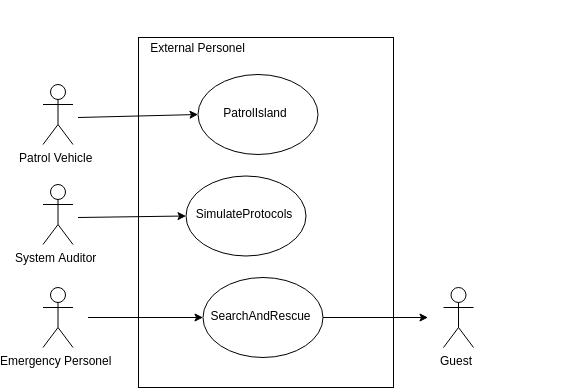
\includegraphics[scale=.30]{Use_Cases__External.png}}
    \caption{Shows the a general view of the External Personnel Use Cases as a diagram.}
    \label{fig:usecaseexternal}
\end{figure}
    \begin{itemize}
        \item[]\textbf{Use Case:}                                
            SearchAndRescue

        \item[]\textbf{Primary Actor:}
            Emergency Personnel

        \item[]\textbf{Goal in Context:}
            To find any potentially remaining guests after a disaster has occurred on the island.
            
        \item[]\textbf{Preconditions:}
            Emergency mode may or may not be currently active, but it has definitely been triggered prior to 
            the arrival of the actor.

        \item[]\textbf{Trigger:}
            A distress signal has been received from Cretaceous Gardens (from Isla Trueno).

        \item[]\textbf{Scenario:}
            \begin{enumerate}
                \item The platoon has received orders to address an emergency on Isla Trueno. 
                \item The troops arrive to the island littered with debris and corpses. 
                \item Some Pay kiosks remain active with an eerie glow coming from an uncannily 
                cheerful welcome screen.
                \item Screams of terror can be heard in the distance, followed by tremendous roars.
                \item The Emergency Personnel head to the kiosks and enter special codes that provide
                them with an enormous supply of token devices.
                \item The EP diffuse throughout the island as they sweep for survivors.
                \item Several helicopters can be heard swarming overhead and small group
                is sent to the CGC Station.
                \item As the troops move inland they find severely injured, but alive, guests.
                \item The troops give the injured new tokens which may be detected by the team
                at the station.
                \item A second group arrives at the island, and is directed by the team at the station
                (via walkie talkies) to the injured.
                \item The team notices the T-Rex Monitor signal moving toward the sweeping group of soldiers
                and they alert them immediately to get into offensive positions.
                \item The helicopters overhead lower themselves to wait for the animal.
                \item Permission to engage is granted and the beast is taken down.
                \item The troops continue their operation until sunrise as teams of paramedics
                are shipped to the island.
            \end{enumerate}

        \item[]\textbf{Exceptions:}
            \begin{itemize}
                \item[] The T.Rex destroys the CGC Station.
            \end{itemize}

        \item[]\textbf{Priority:}
            Essential, must be implemented.
            
        \item[]\textbf{When Available:}
            On demand.

        \item[]\textbf{Frequency of Use:}
            Hopefully never.

        \item[]\textbf{Channel to Primary Actor:}
            Token GPS

        \item[]\textbf{Secondary Actors:}
            Guests, Tokens, Pay Kiosks

        \item[]\textbf{Channels to Secondary Actors:}
            \begin{itemize}
                \item[] Guests: tokens
                \item[] Tokens: pay kiosks
                \item[] Pay Kiosks: direct
            \end{itemize}

        \item[]\textbf{Open Issues:}
            \begin{itemize}
                \item[] None known.
            \end{itemize}
    \end{itemize}
        
    \par\noindent\rule{\textwidth}{0.4pt}  
    \begin{itemize}
        \item[]\textbf{Use Case:}                                
            UpgradeSystemMemory

        \item[]\textbf{Primary Actor:}
            CGC System Technician

        \item[]\textbf{Goal in Context:}
            To upgrade the memory of the machines within at CGC Control Station (e.g. add 16 GB RAM).

        \item[]\textbf{Preconditions:}
            The CGC is not in emergency mode but may be in either maintenance or normal mode.

        \item[]\textbf{Trigger:}
            Cretaceous Gardens experiences an increase in demand, which (if the trend continues) will
            require more computational resources to handle more guests, more efficiently.

        \item[]\textbf{Scenario:}
            \begin{enumerate}
                \item The Sales Department notices a distinct upward trend in sales.
                \item The findings percolate through the relevant business entities within the company.
                \item The CST is dispatched to the Control Station.
                \item The CST enables maintenance mode.
                \item The CST upgrades machines that are currently being used for redundancy.
                \item The CST enables maintenance mode on the redundant machines.
                \item The redundant machines and active machines, switch roles.
                \item The CST upgrades the now-redundant machines.
                \item The CST performs tests.
                \item The CST disables maintenance mode in both active, and redundant machines.
            \end{enumerate}

        \item[]\textbf{Exceptions:}
            \begin{itemize}
                \item[] The trend is ignored by management.
            \end{itemize}

        \item[]\textbf{Priority:}
            Moderate, should be implemented.

        \item[]\textbf{When Available:}
            On demand.

        \item[]\textbf{Frequency of Use:}
            Every two or three fiscal years.

        \item[]\textbf{Channel to Primary Actor:}
            Control station hardware.
        
        \item[]\textbf{Secondary Actors:}
            Sales Department, CGC Control Station, Pay Kiosk
                
        \item[]\textbf{Channels to Secondary Actors:}
            \begin{itemize}
                \item[] Sales Department: pay kiosk transaction logs
                \item[] CGC Control Station: direct access
                \item[] Pay Kiosk: direct connection
            \end{itemize}

        \item[]\textbf{Open Issues:}
            \begin{itemize}
                \item[] None known.
            \end{itemize}
    \end{itemize}

    \par\noindent\rule{\textwidth}{0.4pt}
    \begin{itemize}
        \item[]\textbf{Use Case:}                                
            SimulateProtocols

        \item[]\textbf{Primary Actor:}
            System Auditor

        \item[]\textbf{Goal in Context:}
            To observe currently implemented protocols within the system and provide an analysis
            regarding their safety.

        \item[]\textbf{Preconditions:}
            The system is not in emergency mode nor maintenance mode, but may be put into such
            modes for testing purposes (presumably outside business hours).

        \item[]\textbf{Trigger:}
            The time for a system audit has arrived, either after being scheduled or at random.

        \item[]\textbf{Scenario:}
            \begin{enumerate}
                \item The SA arrives to the CGC Control Station outside of business hours.
                \item The SA requests to observe a simulation of the currently used functions of the system.
                \item The SA is provided with a set of protocols that may be simulated.
                \item For each protocol, the SA runs a simulation.
                \item The system passes the audit and the SA leaves.
                \item OR
                \item The system fails while simulating one or more protocols and the auditor presents a deadline
                to fix the issue lest a fine is incurred.
            \end{enumerate}

        \item[]\textbf{Exceptions:}
            \begin{itemize}
                \item[] An audit occurs in the middle of a system upgrade.
                \item[] The system is triggered into emergency mode (due to an actual emergency)
            \end{itemize}

        \item[]\textbf{Priority:}
            Low, not explicitly required, but may be useful for legal robustness.

        \item[]\textbf{When Available:}
            On demand.

        \item[]\textbf{Frequency of Use:}
            Annually or less frequently.

        \item[]\textbf{Channel to Primary Actor:}
            CGC Control Station interface

        \item[]\textbf{Secondary Actors:}
            CGC Control Station, Pay Kiosks, Cars, Electric Fence, T.Rex, 
            T.Rex Monitor, Camera Network
            
        \item[]\textbf{Channels to Secondary Actors:}
            \begin{itemize}
                \item[] CGC Control Station: simulation
                \item[] Pay Kiosks: simulation
                \item[] Cars: simulation
                \item[] Electric Fence: simulation
                \item[] T.Rex: simulation
                \item[] T.Rex Monitor: simulation
                \item[] Camera Network: simulation
            \end{itemize}

        \item[]\textbf{Open Issues:}
            \begin{itemize}
                \item[] What factors should be relevant in a simulation?
            \end{itemize}
    \end{itemize}
    
    \par\noindent\rule{\textwidth}{0.4pt}
    \begin{itemize}
        \item[]\textbf{Use Case:}                                
            RoutineCheckup

        \item[]\textbf{Primary Actor:}
            Veterinarian

        \item[]\textbf{Goal in Context:}
            To perform a regular physical exam on the T.Rex.

        \item[]\textbf{Preconditions:}
            The T.Rex has been successfully sedated, the veterinarian is completely prepared, 
            the CGC is not in emergency mode, and all components are functioning properly.

        \item[]\textbf{Trigger:}
            The time for a physical has arrived.

        \item[]\textbf{Scenario:}
            \begin{enumerate}
                \item The CGC Station Operator dispatches the veterinarian in a self driving car
                to the edge of the enclosure closest to the current location of the T.Rex.
                \item The veterinarian requests an all-clear confirmation from the operator.
                \item The CGC Station Operator confirms sedated state of the T.Rex.
                \item The operator disengages the electricity of the panel to provide access.
                \item The veterinarian enters and travels toward the animal.
                \item The operator starts a timer.
                \item The veterinarian arrives at the location of the animal.
                \item The operator stops the timer. 
                \item The veterinarian performs a physical exam while the operator provided updates
                on the sedative state of the T.Rex.
                \item The operator alerts the veterinarian when the previously recorded elapsed time
                is approaching the approximated amount of time until the T.Rex wakes up.
                \item The veterinarian concludes the exam.
                \item The veterinarian replenishes the sedative reservoir in the T.Rex Monitor.
                \item The veterinarian travels toward the point of entry.
                \item The veterinarian exits the enclosure.
                \item The Operator confirms successful exit.
                \item The Operator reengages the electricity of the panel.                 
            \end{enumerate}

        \item[]\textbf{Exceptions:}
            \begin{itemize}
                \item[] The T.Rex is found to be in poor health.
                \item[] The sedative lasts less time than expected.
            \end{itemize}

        \item[]\textbf{Priority:}
            Essential, must be implemented.

        \item[]\textbf{When Available:}
            On Demand.

        \item[]\textbf{Frequency of Use:}
            As little as once a year.

        \item[]\textbf{Channel to Primary Actor:}
            \begin{itemize}
                \item[] Enclosure Panel, T.Rex Monitor
            \end{itemize}

        \item[]\textbf{Secondary Actors:}
            CGC Station Operator, T.Rex, Car
        
        \item[]\textbf{Channels to Secondary Actors:}
            \begin{itemize}
                \item[] CGC Station Operator: Car Intercom, Camera Network
                \item[] T.Rex: Enclosure Panel, T.Rex Monitor
            \end{itemize}

        \item[]\textbf{Open Issues:}
            \begin{itemize}
                \item[] Should the panel remain inactive while 
                the veterinarian is inside?
                \item[] Should the veterinarian simply wear an electric 
                safety suit to avoid disengagement all together?
            \end{itemize}
    \end{itemize}
    
    \par\noindent\rule{\textwidth}{0.4pt}    
    \begin{itemize}
        \item[]\textbf{Use Case:} 
            FeedTRex                                

        \item[]\textbf{Primary Actor:}
            Zookeeper

        \item[]\textbf{Goal in Context:}
            To safely provide food for the T.Rex, whether it be live, frozen, thawed, or prepared
            prey.

        \item[]\textbf{Preconditions:}
            The CGC is not in emergency mode, and all components are fully functional.

        \item[]\textbf{Trigger:}
            It is time to feed the T.Rex.

        \item[]\textbf{Scenario:}
            \begin{enumerate}
                \item The CGC Station Operator dispatches the zookeeper in a self driving car
                to the edge of the enclosure furthest from the current location of the T.Rex.
                \item The Zookeeper requests an all-clear confirmation from the operator.
                \item The operator disengages the electricity of the panel to provide access.
                \item The Zookeeper enters and travels a significant distance into the enclosure.
                \item The Zookeeper drops off the food.
                \item The Zookeeper travels back the point of entry.
                \item The Zookeeper exits the enclosure.
                \item The Operator confirms successful exit.
                \item The Operator reengages the electricity of the panel. 
            \end{enumerate}

        \item[]\textbf{Exceptions:}
            \begin{itemize}
                \item[] There is a shortage of food on the island.
                \item[] The T.Rex is sick or injured and does not want to eat.
                \item[] The T.Rex reaches the zookeeper before the zookeeper exits the enclosure.
            \end{itemize}

        \item[]\textbf{Priority:}
            Essential, must be implemented

        \item[]\textbf{When Available:}
            On demand and via operator-zookeeper protocol

        \item[]\textbf{Frequency of Use:}
            Periodically (it can be daily, weekly, or monthly for example)

        \item[]\textbf{Channel to Primary Actor:}
            \begin{itemize}
                \item[] Enclosure Panel
            \end{itemize}

        \item[]\textbf{Secondary Actors:}
            CGC Station Operator, T.Rex, Car
        
        \item[]\textbf{Channels to Secondary Actors:}
            \begin{itemize}
                \item[] CGC Station Operator: Car Intercom, Camera Network
                \item[] T.Rex: Enclosure Panel
            \end{itemize}

        \item[]\textbf{Open Issues:}
            \begin{itemize}
                \item[] Should the panel remain inactive while 
                the zookeeper is inside?
                \item[] Should the zookeeper simply wear an electric 
                safety suit to avoid disengagement all together?
            \end{itemize}
    \end{itemize}
    

\pagebreak
\section{Design Constraints} \label{cons}
\paragraph{} \textit{Due to the real-time nature of the system, there exist some additional 
constraints\footnote{Design Constraints by Anas.}. Namely, it must be the case that all data 
structures concerning the safety controls are as fast as possible but also that they are capable 
of prioritizing all signals in the best way possible.}

    \subsection{Safety}
    \paragraph{} The safety is highly prioritized in our design of the CGC. We have 
    global fire alarm system and the CGC directly have access to it in the case 
    emergency, this event has a very high priority and the CGC 
    should immediately react to this event. When it comes to self-driving cars, we also need to ensure the door locks
    and car should follow appropriate protocol in the case of emergency. For T-Rex, the tranquilizer is a safety precaution which will 
    keep the visitors safe at all times.

    \subsection{Implementation Guidelines}
    \paragraph{} According to the design, we suggest programmers to use some sort of 
    Concurrent safe Messaging Queue for the communication between sensing objects and 
    their associated parent objects. We also recommend using concurrent safe Priority 
    Queue for the CGC, so the CGC can react based on the certain given priority. The 
    priority should be considered because in the case of an emergency, the priority 
    for that event should be at the very top so that the CGC should immediately react 
    to it and follow emergency protocol.

\section{Implementation Plan} \label{impl}
\paragraph{} \textit{There is now a foundation laid out to build something incredible. 
Due to the limitation of time there will only be a small feature set built though. This section will 
ultimately outline the implementation subset that will be delivered during the class period.}\footnote{ Actual Implementation Plan by Siri.}

\paragraph{Overview} To showcase possible behavior that may be seen at the gardens there needs to be a way to showcase 
the GPS tracking of the Visitors, Employees, Cars, and T-rex. The best way to do this is to simulate the actual system 
that would display this information. To do this we will simulate the graphics of the CGC Station which would normally display active nodes
and also act as a way for an employee to control aspects of the system. This simulation will have additional controls that
can control what nodes get spawned into the simulation of the park. The goal for a system like this would be to test the behavior of the protocols 
and also help design protocols. The protocol designer will not be implemented in this version. For now something similar to the following image will be built.
The logic to help make this simulation work will also be built.

\begin{figure}[H]
    \centerline{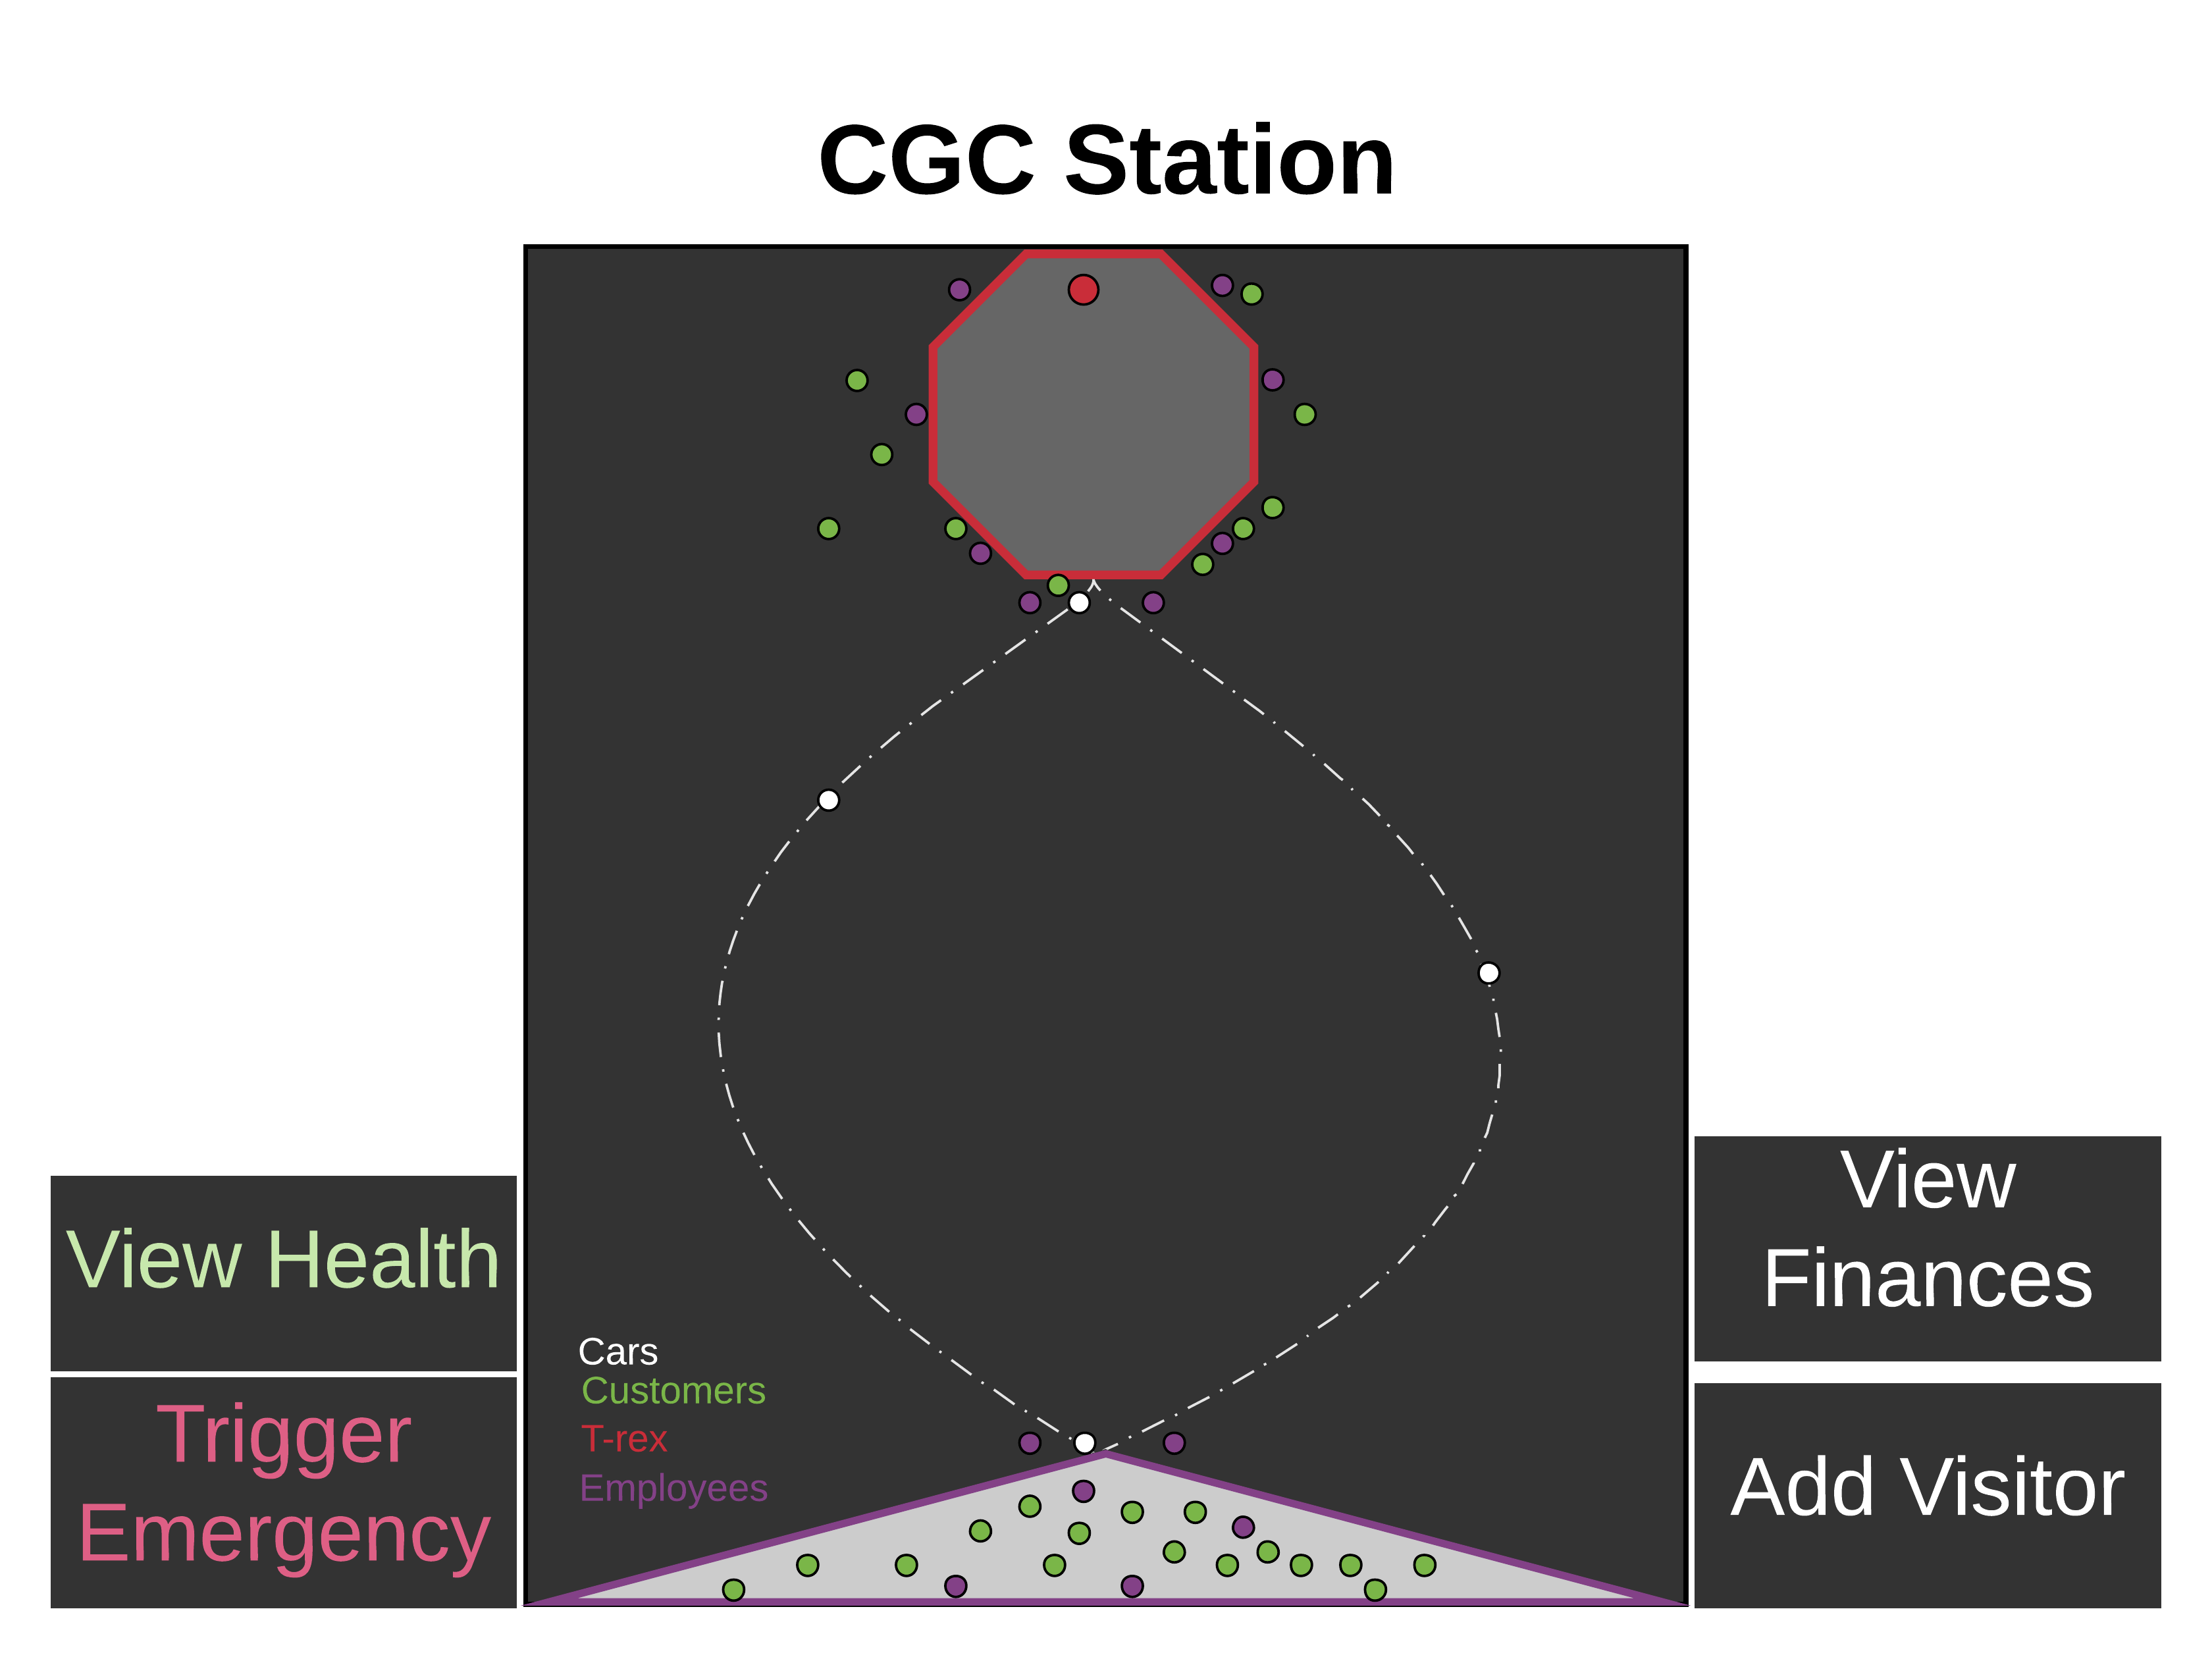
\includegraphics[scale=.10]{CGCStationGUI.png}}
    \caption{\textbf{CGC Station Sim GUI: } A potential version the simulated gui that will be build.}
    \label{fig:CGCStationGUI}
\end{figure}

\paragraph{} To implement this there will be only 5 major classes that will get built and implemented. There 
will be the CGC Station, which includes the GUI, the CGC which will spawn and keep track of the Car, T-Rex Monitor, and Token.
The Car, T-Rex Monitor , and Token will implement the Tracking and Maintainable interface. This will guarantee that 
these classes will report their location and health to the CGC that can then be used to represent this data in a GUI format.
Every class will run on it's own thread. To make these all communicate successfully with eachother, they will all own a Blocking queue. 

\subsection{CGC Station}
\paragraph{} The CGC Station will control the GUI. It will contain a blocking queue and a reference to the CGC blocking queue to communicate. The state of the GUI
will be updated by the CGC by means of messages through the blocking queues.

\subsection{CGC}
\paragraph{} The CGC has its own priority Blocking queue. It has a reference to ALL other active 
instances. It will spawn, manage, and kill other objects and control their threads. 
The goal is to allow a central location to keep track of everything!

\subsection{Car}
\paragraph{} The car will have two versions, the Patrol car and the Tour car. 
The patrol will just go patrol the path to make sure there are no emergencies. The Tour car will implement the logic to pick 
up guests and bring them to the Exhibit and bring them back.

\subsection{T-Rex Monitor}
\paragraph{} This will implement some basic stuff. primarily this exists to show the T-Rex Wondering around in it's cage. 
The T-Rex wondering logic will not be very impressive. the T-Rex will not attempt to get out or 
hurt guests. when emergency mode is triggered, 
it may act like it got injected with a tranq. This will just make the movement stop.

\subsection{Token}
\paragraph{} This will be used to showcase the GPS location on the map for the visitors and the Employees. It will have very basic behavior one 
to make it move towards the car pickup location on the south lot. It will also wonder around looking at the dinasour until time is up.

\subsection{Pay Kiosk}
\paragraph{} This will randomly make sails and spawn visitors intot he simulation. and log the transactions.

\paragraph{}Every class will extend or implement the animation timer to allow it to perform behavior against time. For example, 
to give a realistic pace to the movement of a token GPS. the X and Y location of the gps may not move every frame. The animation timer is what allows this animation of data.
the only class that will NOT extend an animation timer is the CGC this class will respond only to messages in its blocking queue. It will wait other wise.

\subsection{Details}
\paragraph{}To implement this in the 3 week period we will stratigically implement the basic functioning of the software product. If we have time,
 we will add additional features. The goal is to showcase something. Hopefully we can showcase a lot. The next tabel describes the goals for each
 week and what to accomplish 

\begin{table}[H]
\begin{tabularx}{\hsize}{|X|X|}
    \hline
    \rowcolor{LightBlue}
    \multicolumn{2}{|c|}{\textbf{Work Schedule }} \\
    \hline
    \textbf{Week} & \textbf{Goals} \\
    \hline
    \center \textbf{Week 1} & 
        \begin{itemize}
            \item Build all skeleton classes
            \item Assign tasks from LoboGit
            \item Begin to code
        \end{itemize} \\
    \hline
        \center \textbf{Week 2} & 
        \begin{itemize}
            \item Complete basic implementation
            \item Check team task progress
            \item Assign  NEW tasks from LoboGit
            \item Continue to code
            \item Fix Bugs
            \item Complete ReadMe file
        \end{itemize} \\
    \hline
        \center \textbf{Week 3} & 
        \begin{itemize}
            \item Add final touches to features
            \item Fix final bugs
            \item list known issues in ReadMe 
            \item Go over presentation details
        \end{itemize} \\
    \hline
\end{tabularx}
\end{table}

\section{Definition of Terms} \label{defs}
\paragraph{} \textit{The following is a list of definitions contain the most commonly used 
technical terms within this document, whose meaning may not be immediately apparent to the 
lay reader. Most definitions are defined by the authors for use within the context of this 
document. Some may originate from vocabulary shared across the general references cited \nocite{*}. 
In the event that a definition was taken directly from a source, it is followed by a citation.
\footnote{This list is mostly a reduction of the term list found in the preceding Software 
Design Specification document.}}

\begin{list}{}{}
    \item \textbf{CGC:} Cretaceous Gardens Controller 
    \item \textbf{DVR:} Digital Video Recorder
    \item \textbf{Electrical Conduction:} The movement of electrically charged particles through a transmission medium.
    \item \textbf{GPS:} Global Positioning System 
    \item \textbf{Hardwired Ethernet:} This references the latest IEEE standard for Ethernet utilizing physical cables.
    \item \textbf{Network:} All nodes with which the CGC interacts, the links that connect them to each other and to the CGC, the CGC itself, and all related databases.
    \item \textbf{Node:} The generic term that refers to any device connected to the CGC in any way. This includes autonomous vehicles, tokens, the T.Rex monitor, all electric fence panels, all kiosks, and all cameras.
    \item \textbf{Safely Inactive:} A state in which a vehicle is fully functional and ready to be dispatched.
    \item \textbf{Safely Occupied:} A state in which a vehicle contains at least one person, is locked, and is ready to depart.
    \item \textbf{Token:} An interactive device used by the visitor that grants access to locations.
\end{list}
\pagebreak
\bibliography{../../ReferenceMaterial/BibTeX/references}
% run latex, then bibtex, then quickbuild (on the tex file)
\end{document}
